%%%%%%%%%%%%%%%%%%%%%%%%%%%%%%%%%%%%%%%%%
% Short Sectioned Assignment LaTeX Template Version 1.0 (5/5/12)
% This template has been downloaded from: http://www.LaTeXTemplates.com
% Original author:  Frits Wenneker (http://www.howtotex.com)
% License: CC BY-NC-SA 3.0 (http://creativecommons.org/licenses/by-nc-sa/3.0/)
%%%%%%%%%%%%%%%%%%%%%%%%%%%%%%%%%%%%%%%%%

%----------------------------------------------------------------------------------------
%	PACKAGES AND OTHER DOCUMENT CONFIGURATIONS
%----------------------------------------------------------------------------------------

\documentclass[paper=a4, fontsize=11pt]{scrartcl} % A4 paper and 11pt font size

% ---- Entrada y salida de texto -----

\usepackage{hyperref}
\usepackage{varioref}
\usepackage[T1]{fontenc} % Use 8-bit encoding that has 256 glyphs
\usepackage[utf8]{inputenc}
%\usepackage{fourier} % Use the Adobe Utopia font for the document - comment this line to return to the LaTeX default

% ---- Idioma --------

\usepackage[spanish, es-tabla]{babel} % Selecciona el español para palabras introducidas automáticamente, p.ej. "septiembre" en la fecha y especifica que se use la palabra Tabla en vez de Cuadro

% ---- Otros paquetes ----

\usepackage{amsmath,amsfonts,amsthm} % Math packages
%\usepackage{graphics,graphicx, floatrow} %para incluir imágenes y notas en las imágenes
\usepackage{graphics,graphicx, float} %para incluir imágenes y colocarlas

% Para hacer tablas comlejas
%\usepackage{multirow}
%\usepackage{threeparttable}

%\usepackage{sectsty} % Allows customizing section commands
%\allsectionsfont{\centering \normalfont\scshape} % Make all sections centered, the default font and small caps

\usepackage{fancyhdr} % Custom headers and footers
\pagestyle{fancyplain} % Makes all pages in the document conform to the custom headers and footers
\fancyhead{} % No page header - if you want one, create it in the same way as the footers below
\fancyfoot[L]{} % Empty left footer
\fancyfoot[C]{} % Empty center footer
\fancyfoot[R]{\thepage} % Page numbering for right footer
\renewcommand{\headrulewidth}{0pt} % Remove header underlines
\renewcommand{\footrulewidth}{0pt} % Remove footer underlines
\setlength{\headheight}{13.6pt} % Customize the height of the header

\numberwithin{equation}{section} % Number equations within sections (i.e. 1.1, 1.2, 2.1, 2.2 instead of 1, 2, 3, 4)
\numberwithin{figure}{section} % Number figures within sections (i.e. 1.1, 1.2, 2.1, 2.2 instead of 1, 2, 3, 4)
\numberwithin{table}{section} % Number tables within sections (i.e. 1.1, 1.2, 2.1, 2.2 instead of 1, 2, 3, 4)

\setlength\parindent{0pt} % Removes all indentation from paragraphs - comment this line for an assignment with lots of text

\newcommand{\horrule}[1]{\rule{\linewidth}{#1}} % Create horizontal rule command with 1 argument of height


%----------------------------------------------------------------------------------------
%	TÍTULO Y DATOS DEL ALUMNO
%----------------------------------------------------------------------------------------

\title{	
\normalfont \normalsize 
\textsc{{\bf Ingeniería de Servidores (2015-2016)} \\ Grado en Ingeniería Informática \\ Universidad de Granada} \\ [25pt] % Your university, school and/or department name(s)
\horrule{0.5pt} \\[0.4cm] % Thin top horizontal rule
\huge Memoria Práctica 2 \\ % The assignment title
\horrule{2pt} \\[0.5cm] % Thick bottom horizontal rule
}

\author{Francisco Carrillo Pérez} % Nombre y apellidos

\date{\normalsize\today} % Incluye la fecha actual

%----------------------------------------------------------------------------------------
% DOCUMENTO
%----------------------------------------------------------------------------------------

\begin{document}

\maketitle % Muestra el Título

\newpage %inserta un salto de página

\tableofcontents % para generar el índice de contenidos

\listoffigures

\listoftables

\newpage

%%%%%%%%%%%%%%%%%%%%%%%%%%%%%%%%%%%%%%%%%%%%%%%%%%%%
% CUESTIÓN 1
%%%%%%%%%%%%%%%%%%%%%%%%%%%%%%%%%%%%%%%%%%%%%%%%%%%%
\section{Cuestión 1: Liste los argumentos de yum necesarios para instalar, buscar y eliminar paquetes}
Según la documentación de CentOS \cite{yum1} \cite{yum2}:\\
Para instalar nuevos paquetes utilizaremos: \textbf{su -c 'yum install packagename'}.\\
Para buscar nuevos paquetes utilizaremos: \textbf{su -c 'yum search packagename'}.\\
Para eliminar paquetes utilizaremos: \textbf{su -c 'yum remove packagename'}.\\
Por lo tanto los argumentos serían:

\begin{itemize}
	\item Instalar: install
	\item Buscar: search
	\item Eliminar: remove
\end{itemize}

%%%%%%%%%%%%%%%%%%%%%%%%%%%%%%%%%%%%%%%%%%%%%%%%%%%%
% CUESTIÓN 2
%%%%%%%%%%%%%%%%%%%%%%%%%%%%%%%%%%%%%%%%%%%%%%%%%%%%

\section{Cuestión 2:}
\subsection{ ¿Qué ha de hacer para que yum tenga acceso a Internet?}
Según la página de documentación de CentOS \cite{yum-proxy} para que yum tenga acceso a internet tenemos que:\\
Tenemos que especificar los detalles del proxy en el archivo /etc/yum.conf .
Dentro del archivo escribimos:\\
proxy= astargate.ugr.es:3128\\
\subsection{¿Cómo añadimos un nuevo repositorio?}
Para añadir un nuevo repositorio según la documentación de CentOS \cite{anadirrepositorio}:\\
\textbf{su -c 'cp example.repo /etc/yum.repos.d/'}

%%%%%%%%%%%%%%%%%%%%%%%%%%%%%%%%%%%%%%%%%%%%%%%%%%%%
% CUESTIÓN 3
%%%%%%%%%%%%%%%%%%%%%%%%%%%%%%%%%%%%%%%%%%%%%%%%%%%%

\section{Cuestión 3: Indique el comando para buscar un paquete en un repositorio y el correspondiente para instalarlo}
El comando para buscar un paquete en un repositorio es \cite{apt-search}:\\
\textbf{apt-cache search $<$término$>$}\\
El comando para instalar un paquete es \cite{apt-search}:\\
\textbf{apt-get install $<$paquete$>$}\\
Aunque en nuevas versiones, se puede utilizar solo apt, sin la necesidad de añadir el get o el cache.

\begin{figure}[H] %con el [H] le obligamos a situar aquí la figura
	\centering
	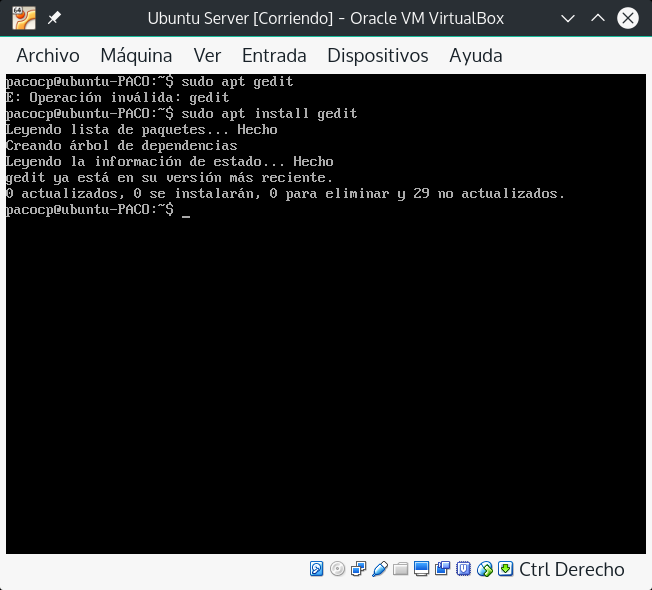
\includegraphics[scale=0.5]{figuras/figura30.png}  %el parámetro scale permite agrandar o achicar la imagen. En el nombre de archivo puede especificar directorios
	\label{figura30}
	
	\caption{Vemos como podemos instalar solo con apt} 
\end{figure}

%%%%%%%%%%%%%%%%%%%%%%%%%%%%%%%%%%%%%%%%%%%%%%%%%%%%
% CUESTIÓN 4
%%%%%%%%%%%%%%%%%%%%%%%%%%%%%%%%%%%%%%%%%%%%%%%%%%%%

\section{Cuestión 4: Indique qué ha modificado para que apt pueda acceder a los servidores de paquetes a través del proxy. ¿Cómo añadimos un nuevo repositorio?}
Para poder acceder a los paquetes a través del proxy siguiendo la página de ayuda de Ubuntu\cite{apt-proxy}:\\
\begin{itemize}
	\item Abrimos el archivo /etc/apt/apt.conf con root: 	\textbf{sudo editorfavorito /etc/apt/apt.conf}
	\item Y añadimos esta línea: \textbf{Acquire::http::Proxy "astargate.ugr.es:3128";}
\end{itemize}
Para añadir un repositorio tenemos dos opciones \cite{apt-repositorie}:
\begin{itemize}
	\item Si son repositorios universisales que ya vienen en el archivo  /etc/apt/sources.list podemos usarlos descomentandolos en ese archivo, o utilizando la orden: \textbf{sudo add-apt-repository "deb http://us.archive.ubuntu.com/ubuntu/ saucy universe multiverse"}
	\item Si son repositorios PPA utilizamos la orden: \textbf{sudo add-apt-repository ppa:<repository-name>}
\end{itemize}

%%%%%%%%%%%%%%%%%%%%%%%%%%%%%%%%%%%%%%%%%%%%%%%%%%%%
% CUESTIÓN 5
%%%%%%%%%%%%%%%%%%%%%%%%%%%%%%%%%%%%%%%%%%%%%%%%%%%%

\section{Cuestión 5: ¿Qué diferencia hay entre telnet y ssh?}
Leyendo la documentación de la Wikipedia de ambos proyectos \cite{telnet1} \cite{ssh1} la clara diferencia es en cuanto a la seguridad:\\
Mientras que el protocolo telnet no encripta nada de los datos que se envían por las conexiones, ni si quiera las contraseñas, además de que no tiene ninguna autentificación para comprobar que la conexión es segura, mientras que el protocolo ssh todos los envíos son encriptados y utiliza una llave pública encriptada para comprobar al ordenador remoto.
%%%%%%%%%%%%%%%%%%%%%%%%%%%%%%%%%%%%%%%%%%%%%%%%%%%%
% CUESTIÓN 6
%%%%%%%%%%%%%%%%%%%%%%%%%%%%%%%%%%%%%%%%%%%%%%%%%%%%

\section{Cuestión 6: ¿Para que sirve la opción -X?}
Según la página del man de ssh \cite{-X}:\\
La opción -X permite activar el reenvío de X11.
Cuando intentamos ejecutar gedit abriendo la sesión con ssh IP: 
\begin{figure}[H] %con el [H] le obligamos a situar aquí la figura
	\centering
	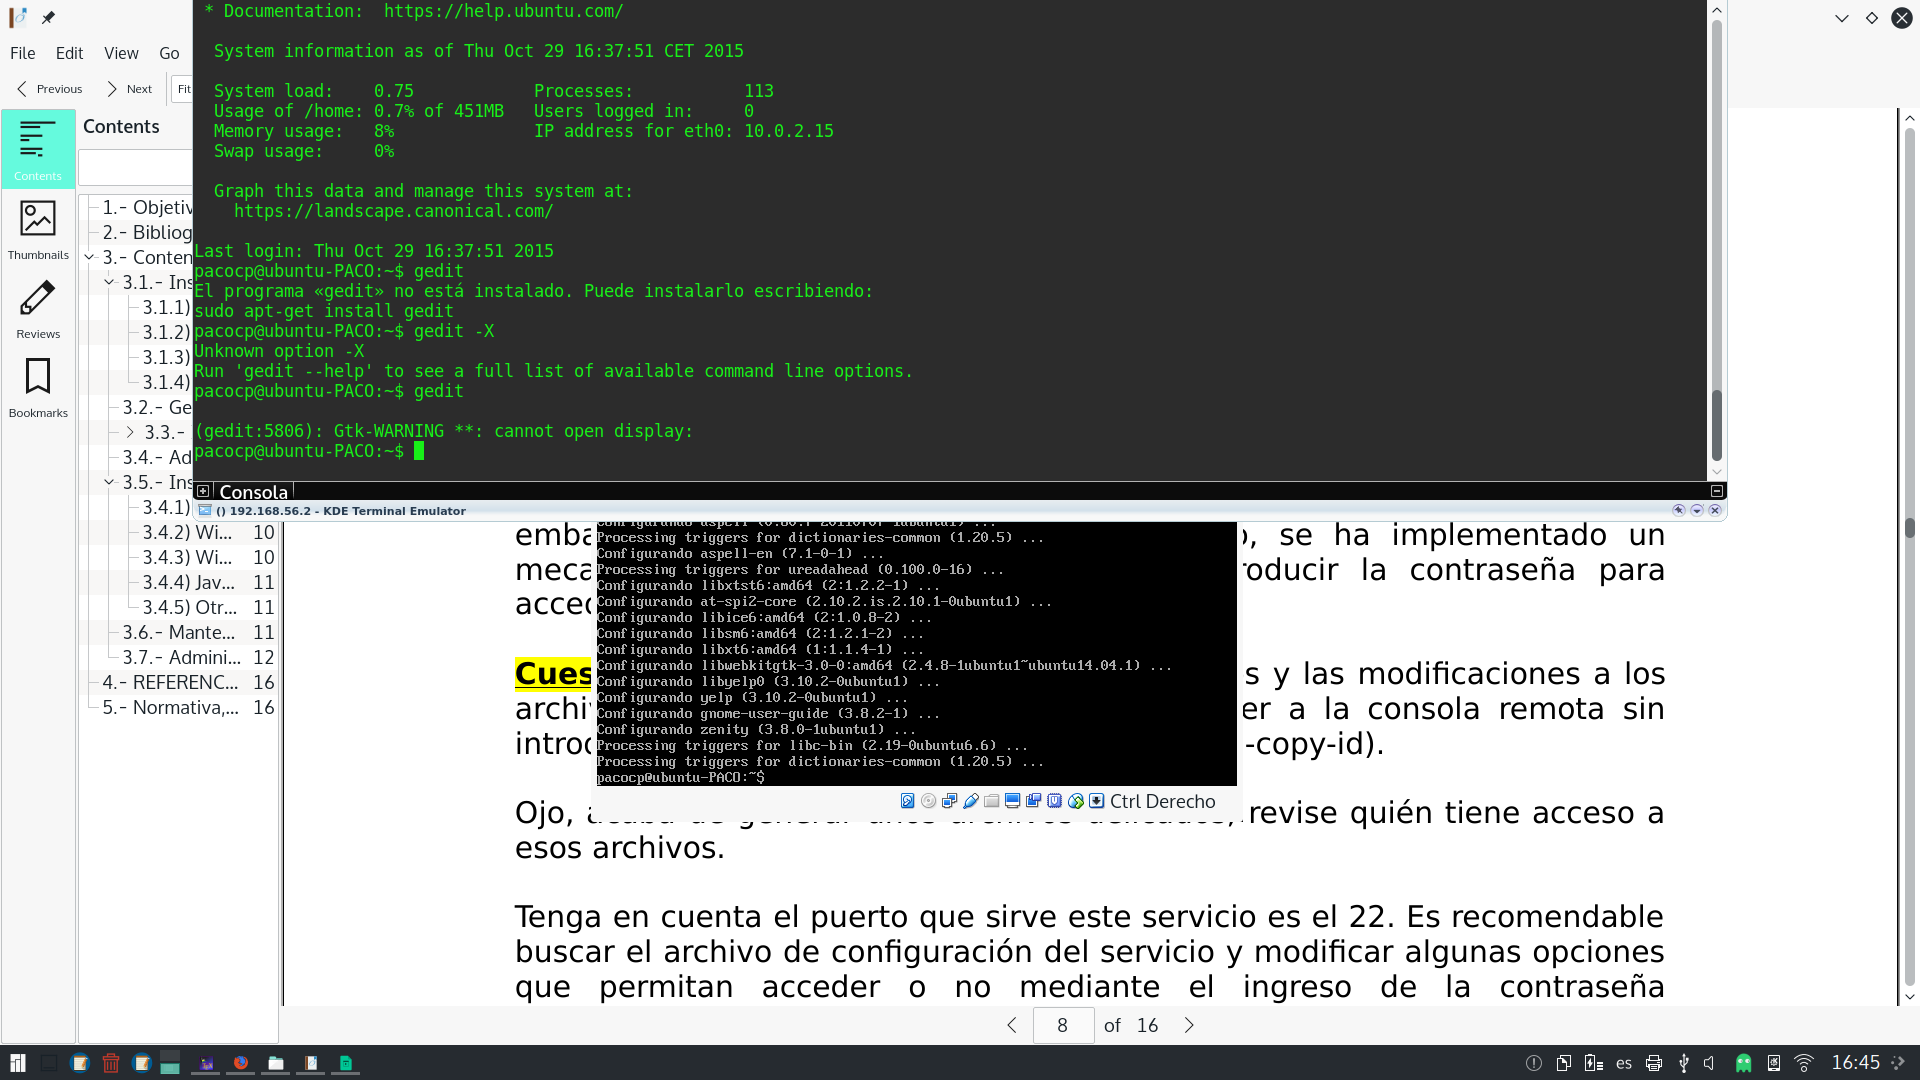
\includegraphics[scale=0.3]{figuras/figura1.png}  %el parámetro scale permite agrandar o achicar la imagen. En el nombre de archivo puede especificar directorios
	\label{figura1}
	
	\caption{Fallo al intentar ejecutar gedit abriendo la sesión con: ssh IP} 
\end{figure}
El error nos indica que no puede cargar la interfaz gráfica GTK.
En cambio si abrimos la sesión con la opción -X:
\begin{figure}[H] %con el [H] le obligamos a situar aquí la figura
	\centering
	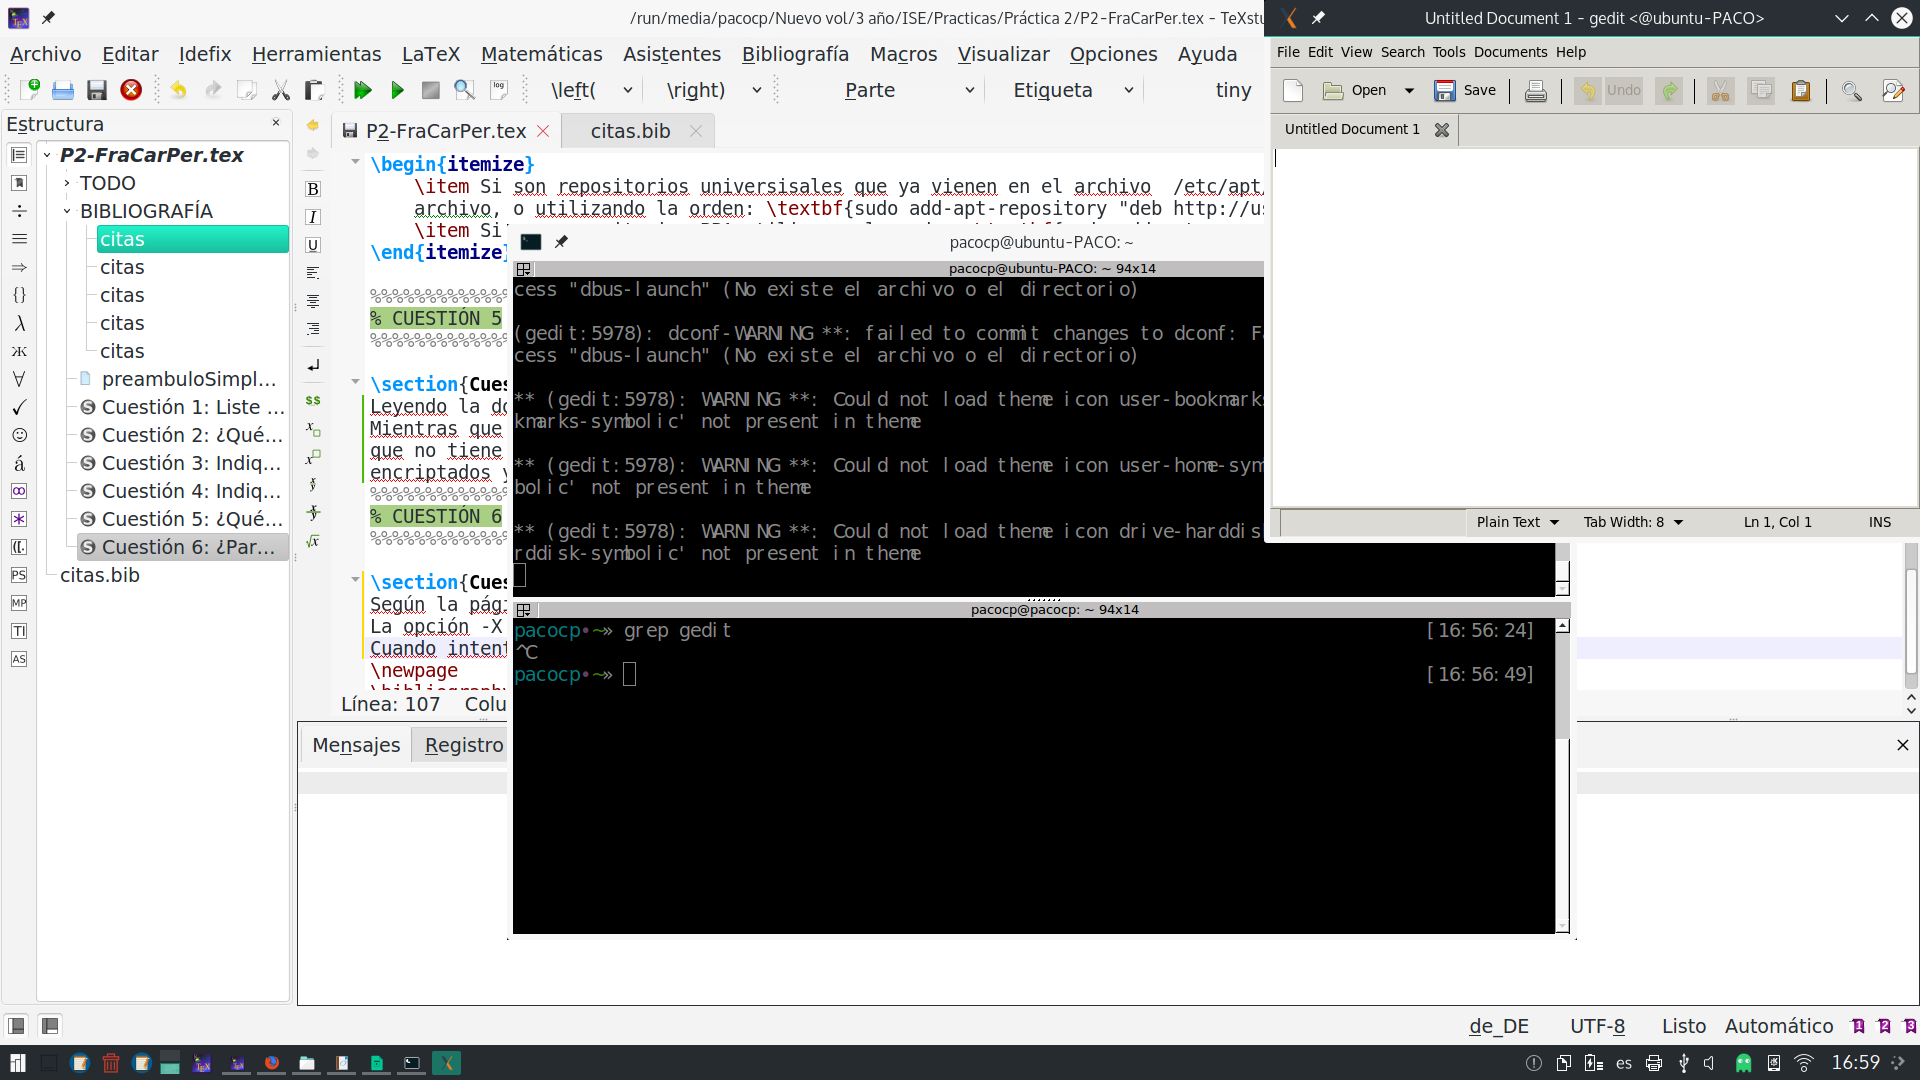
\includegraphics[scale=0.3]{figuras/figura3.png}  %el parámetro scale permite agrandar o achicar la imagen. En el nombre de archivo puede especificar directorios
	\label{figura3}
	
	\caption{Podemos comprobar que se carga gedit abriendo la sesión con: ssh -X IP} 
\end{figure}
%%%%%%%%%%%%%%%%%%%%%%%%%%%%%%%%%%%%%%%%%%%%%%%%%%%%
% CUESTIÓN 7
%%%%%%%%%%%%%%%%%%%%%%%%%%%%%%%%%%%%%%%%%%%%%%%%%%%%


\section{Cuestión 7: Muestre la secuencia de comandos y las modificaciones a los archivos correspondientes para permitir acceder a la consola remota sin introducir contraseñas.}
Para conseguirlo debemos seguir los siguientes pasos \cite{ssh-keygen} \cite{ssh-copy-id} \cite{tuto}:
\begin{enumerate}
	\item En la máquina local (en mi caso una máquina con Manjaro \cite{manjaro} instalado) ejecutamos el comando ssh-keygen para generar unas claves públicas.
		\textbf{ssh-keygen}
	\item Vamos a observar los permisos que tienen los archivos que se han generado con el comando:	
		\textbf{ls -la .ssh$/$}
	\item Le cambiamos los permisos para que sólo sean de lectura y escritura por el grupo, con el comando:
		\textbf{chmod 600 /.ssh/id\_rsa.}
	\item En el archivo de configuración del ssh en el servidor con el comando: 
		\textbf{vi $/$etc$/$ssh$/$sshd\_config}\\
		Descomentamos la línea: PasswordAuthentication yes
	\item Con el comando ssh-copy-id copiamos la clave pública al nombre del host. (En mi caso he utilizado la IP del servidor ).
		\textbf{ssh-copy-id  192.168.56.2}
\end{enumerate}

\begin{figure}[H] %con el [H] le obligamos a situar aquí la figura
	\centering
	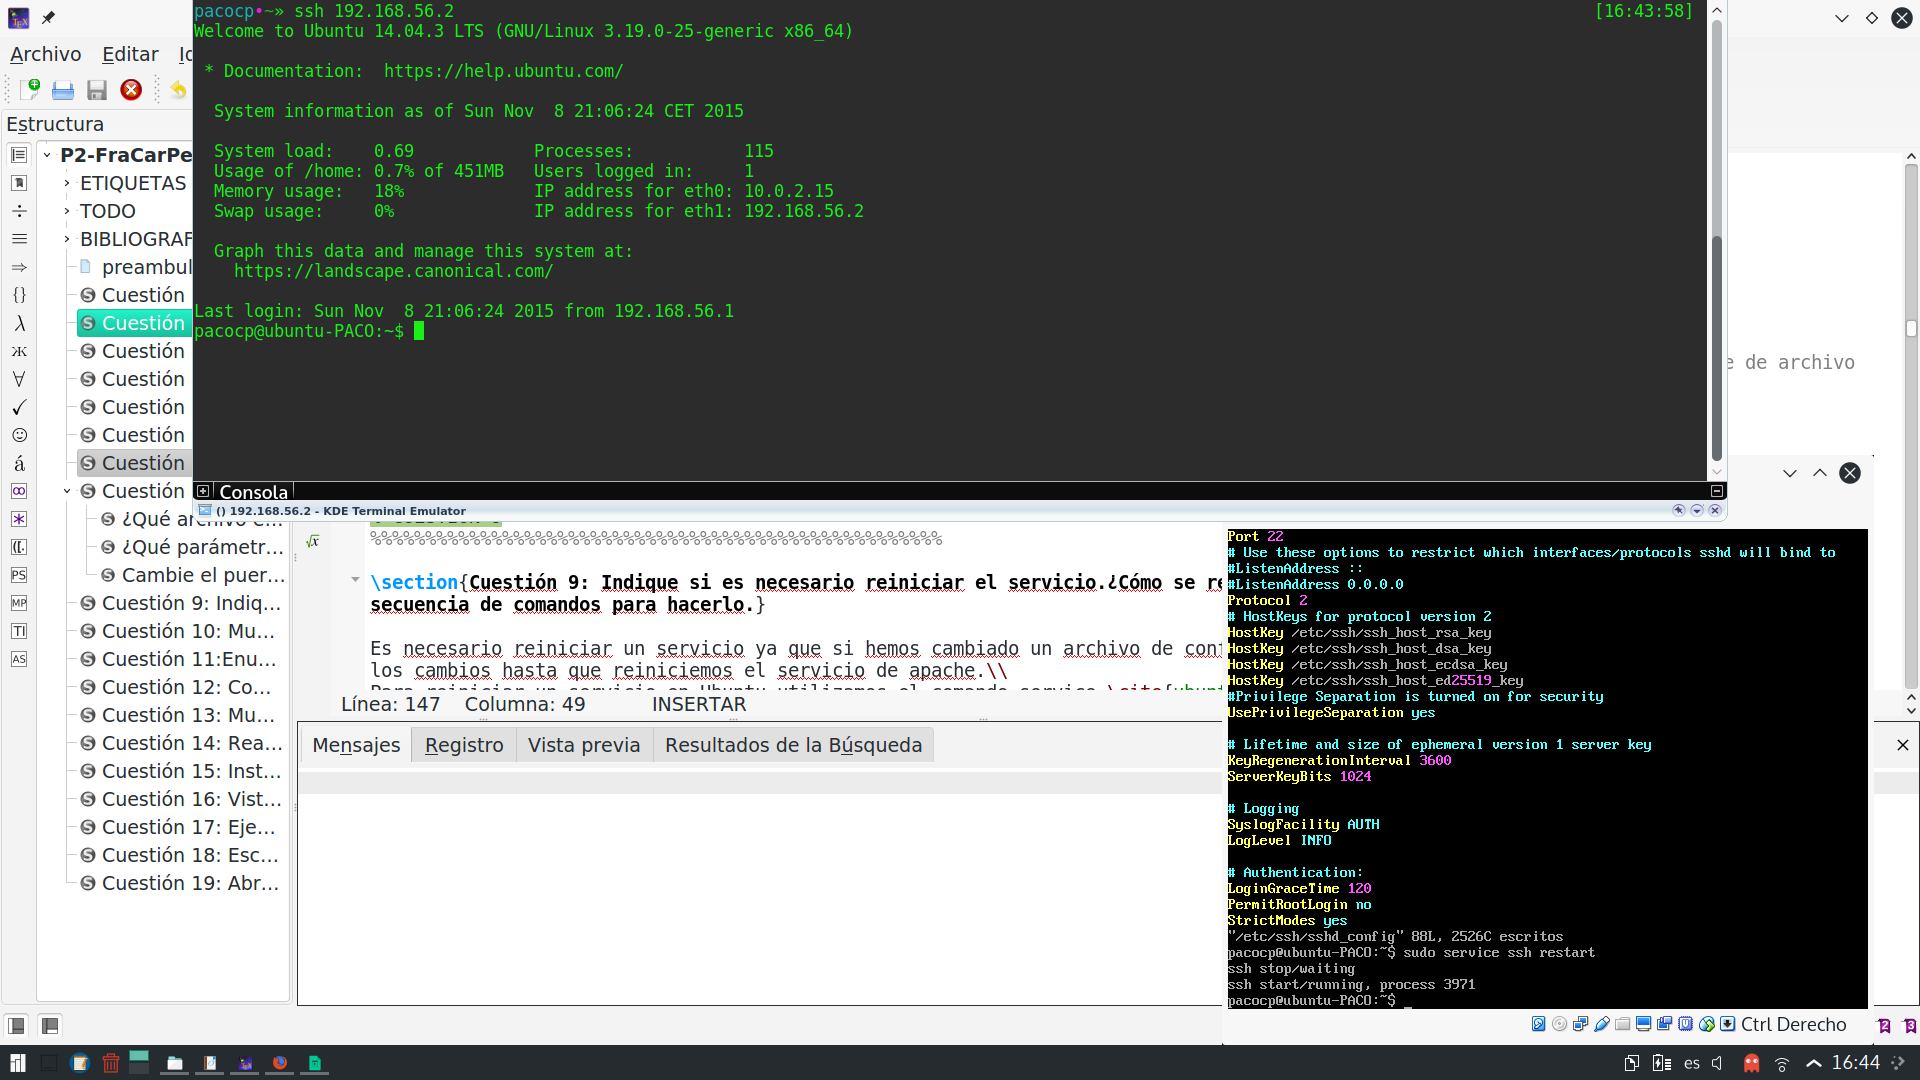
\includegraphics[scale=0.3]{figuras/figura31.png}  %el parámetro scale permite agrandar o achicar la imagen. En el nombre de archivo puede especificar directorios
	\label{figura31}
	
	\caption{Podemos comprobar cómo no me pide la contraseña para entrar} 
\end{figure}
%%%%%%%%%%%%%%%%%%%%%%%%%%%%%%%%%%%%%%%%%%%%%%%%%%%%
% CUESTIÓN 8
%%%%%%%%%%%%%%%%%%%%%%%%%%%%%%%%%%%%%%%%%%%%%%%%%%%%

\section{Cuestión 8:   }
\subsection{¿Qué archivo es el que contiene la configuración de sshd?}
El archivo que contiene la confuguración del sshd es:\\
\textbf{$/$etc$/$ssh$/$sshd\_config}
\subsection{¿Qué parámetro hay que modificar para evitar que el usuario root acceda?}
Si bajamos por el archivo veremos la línea:\\
\textbf{PermitRootLogin without-password}\\
Esa línea la cambiamos por:\\
\textbf{PermitRootLogin no}\\
Y reiniciamos el servicio del ssh para que se apliquen los cambios:\\
\textbf{service ssh restart}
\subsection{Cambie el puerto por defecto y compruebe que puede acceder.}
Para cambiar el puerto por defecto justo en la cabecera del archivo vemos:\\
\textbf{Port 22}\\
Y lo cambiamos por:\\
\textbf{Port 25}\\
Y reiniciamos el servicio del ssh para que se apliquen los cambios:\\
\textbf{service ssh restart}

\begin{figure}[H] %con el [H] le obligamos a situar aquí la figura
	\centering
	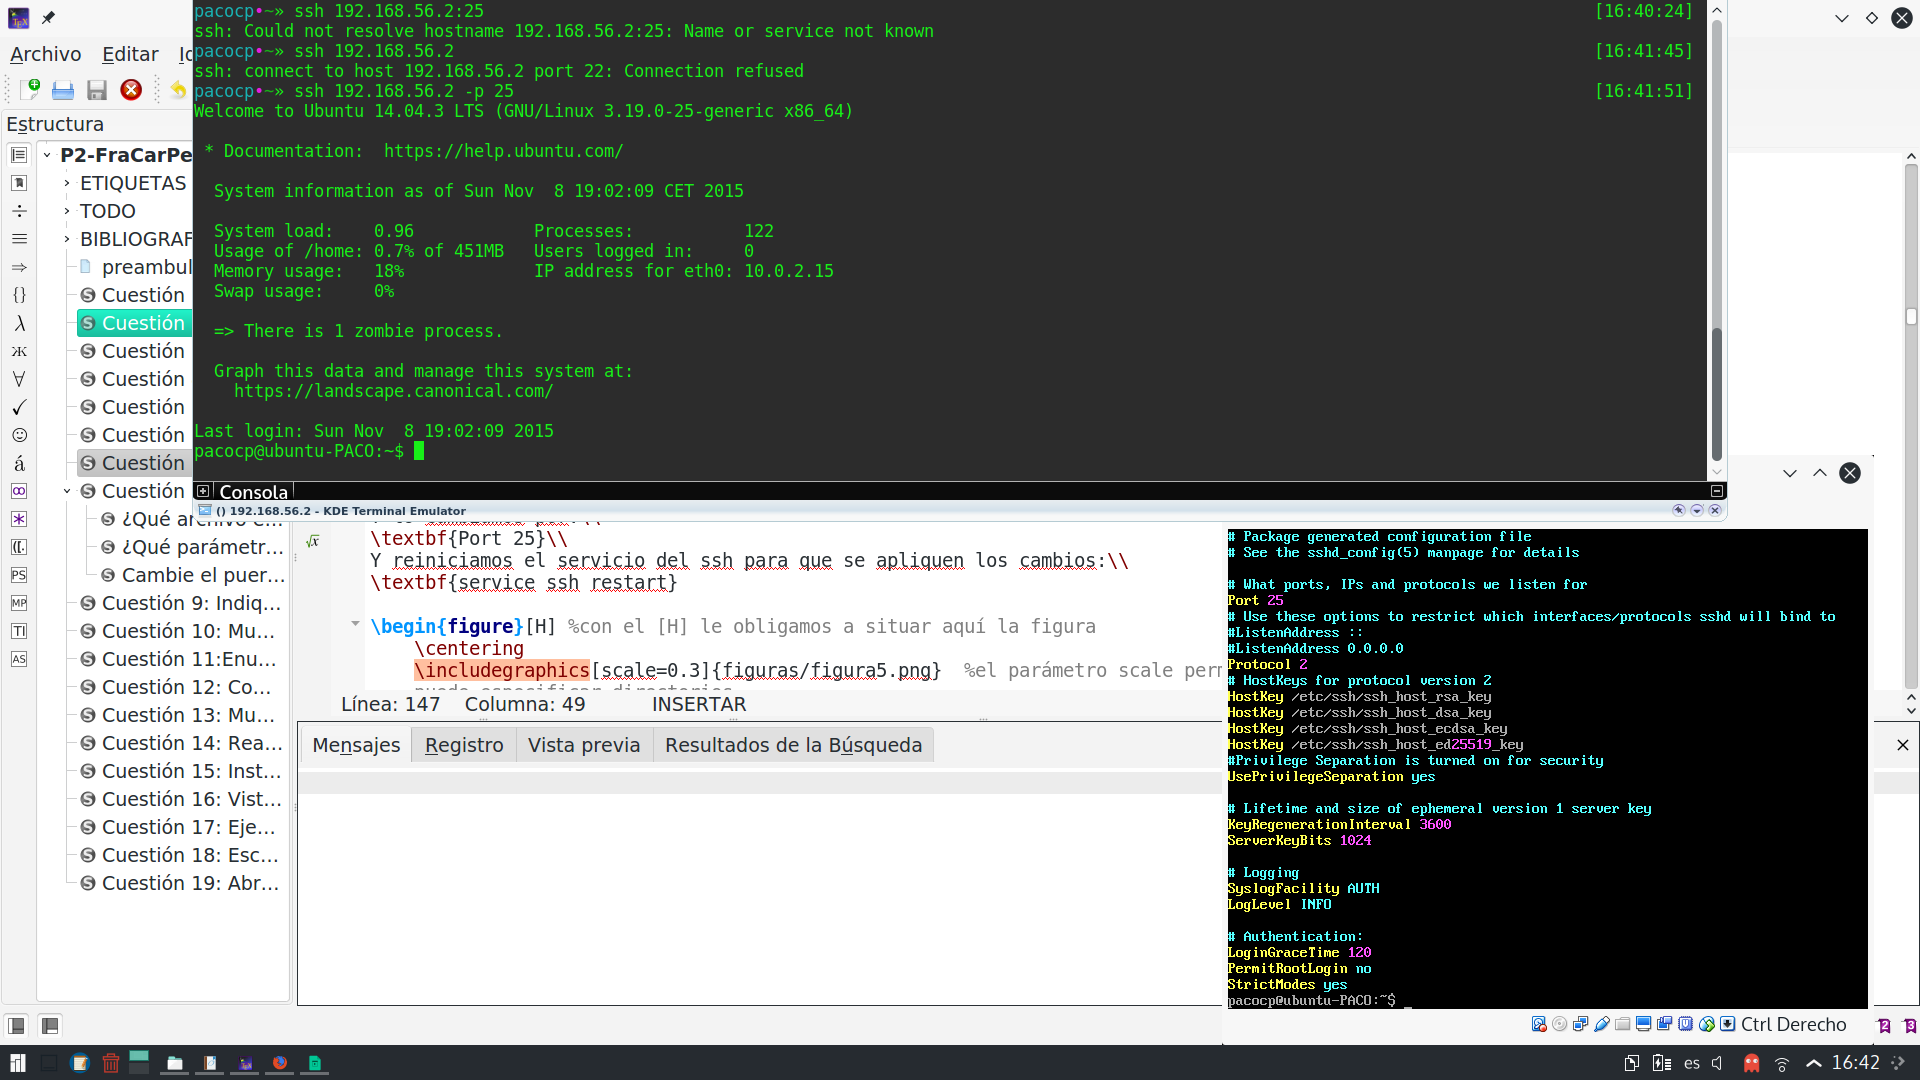
\includegraphics[scale=0.3]{figuras/figura5.png}  %el parámetro scale permite agrandar o achicar la imagen. En el nombre de archivo puede especificar directorios
	\label{figura5}
	
	\caption{Podemos comprobar como he cambiado el puerto y sigo podiendo conectarme, pero necesito espeficarle el puerto con la opción \textbf{-p 25}} 
\end{figure}
%%%%%%%%%%%%%%%%%%%%%%%%%%%%%%%%%%%%%%%%%%%%%%%%%%%%
% CUESTIÓN 9
%%%%%%%%%%%%%%%%%%%%%%%%%%%%%%%%%%%%%%%%%%%%%%%%%%%%

\section{Cuestión 9: Indique si es necesario reiniciar el servicio.¿Cómo se reinicia un servicio en Ubuntu?¿y en CentOS? Muestre la secuencia de comandos para hacerlo.}

Es necesario reiniciar un servicio ya que si hemos cambiado un archivo de configuración, por ejemplo el php.ini, no se verían reflejados los cambios hasta que reiniciemos el servicio de apache.\\
Para reiniciar un servicio en Ubuntu utilizamos el comando service \cite{ubuntu-restart}:\\
\textbf{service nombredelservicio restart}\\
Para reiniciar un servicio en CentOS se realiza de la siguiente manera \cite{centOS-restart}:\\
\textbf{systemctl nombredelservicio restart}\\

%%%%%%%%%%%%%%%%%%%%%%%%%%%%%%%%%%%%%%%%%%%%%%%%%%%%
% CUESTIÓN 10
%%%%%%%%%%%%%%%%%%%%%%%%%%%%%%%%%%%%%%%%%%%%%%%%%%%%

\section{Cuestión 10: Muestre los comandos que ha utilizado en Ubuntu Server y en CentOS }

Vamos a ver los pasos que he seguido para instalar Apache + MySQL + Python y PHP en Ubuntu Server:
\begin{enumerate}
	\item Instalamos apache con el comando \cite{apache}: \textbf{sudo apt-get install apache2}
	\item Instalamos MySQL con el comando \cite{mysql}: \textbf{sudo apt-get install mysql-server}
	\item Por último, Python viene preinstalado en Ubuntu Server, como podemos comprobar en \ref{figura4}
	También vamos a instalar PHP para poder continuar con la instalacion de phpMyAdmin en la pregunta \ref{cuestion15} con los siguientes comandos:\\
	\textbf{sudo apt-get install php5 libapache2-mod-php5}\\
	Para poder usar PHP con MySQL es:\\
	\textbf{sudo apt-get install php5-mysql}
\end{enumerate}

\begin{figure}[H] %con el [H] le obligamos a situar aquí la figura
	\centering
	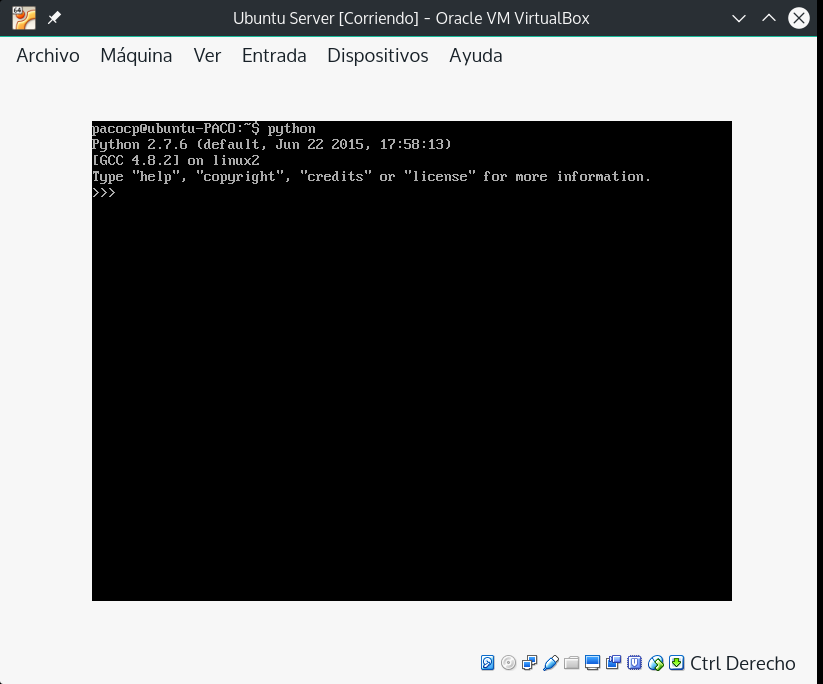
\includegraphics[scale=0.3]{figuras/figura4.png}  %el parámetro scale permite agrandar o achicar la imagen. En el nombre de archivo puede especificar directorios
	\label{figura4}
	
	\caption{Podemos observar como Python se encuentra instalado} 
\end{figure}

 Ahora, vamos a ver los pasos para instalar Apache + MySQL + PHP y Python en CentOS \cite{lamp-centOs}.
 \begin{enumerate}
 	\item Instalamos Apache con el comando: \textbf{sudo yum install httpd} \\
		  Además tenemos que hacerle un start al servicio con: \textbf{systemctl start httpd.service}
	\item Para instalar MySQL usamos el comando: \textbf{sudo yum install mariadb-server mariadb} \\
		  Además tenemos que hacerle un start al servicio con : \textbf{sudo systemctl start mariadb}
	\item Por último vamos a instalar PHP y Python:\\
		  \textbf{sudo yum install php php-mysql} \\
		  Reiniciamos el servicio:\textbf{sudo systemctl restart httpd.service} \\
		  Para instalar Python:\\
		  \textbf{sudo yum install python}
 \end{enumerate}
%%%%%%%%%%%%%%%%%%%%%%%%%%%%%%%%%%%%%%%%%%%%%%%%%%%%
% CUESTIÓN 11
%%%%%%%%%%%%%%%%%%%%%%%%%%%%%%%%%%%%%%%%%%%%%%%%%%%%

\section{Cuestión 11:Enumere otros servidores web y las páginas de sus proyectos (mínimo 3 sin considerar Apache, IIS ni nginx)}
\begin{itemize}
	\item \textbf{Cherokee Web Server} \cite{cherokee}
	\item \textbf{Lighttpd} \cite{lighttpd}
	\item \textbf{IBM HTTP Server} \cite{ibm-server}
\end{itemize}

%%%%%%%%%%%%%%%%%%%%%%%%%%%%%%%%%%%%%%%%%%%%%%%%%%%%
% CUESTIÓN 12
%%%%%%%%%%%%%%%%%%%%%%%%%%%%%%%%%%%%%%%%%%%%%%%%%%%%

\section{Cuestión 12: Compruebe que el servicio está funcionando accediendo a la MV a través de la anfitriona.}
Primero tengo que configurar la red Host-Only \ref{figura6}:
\begin{figure}[H] %con el [H] le obligamos a situar aquí la figura
	\centering
	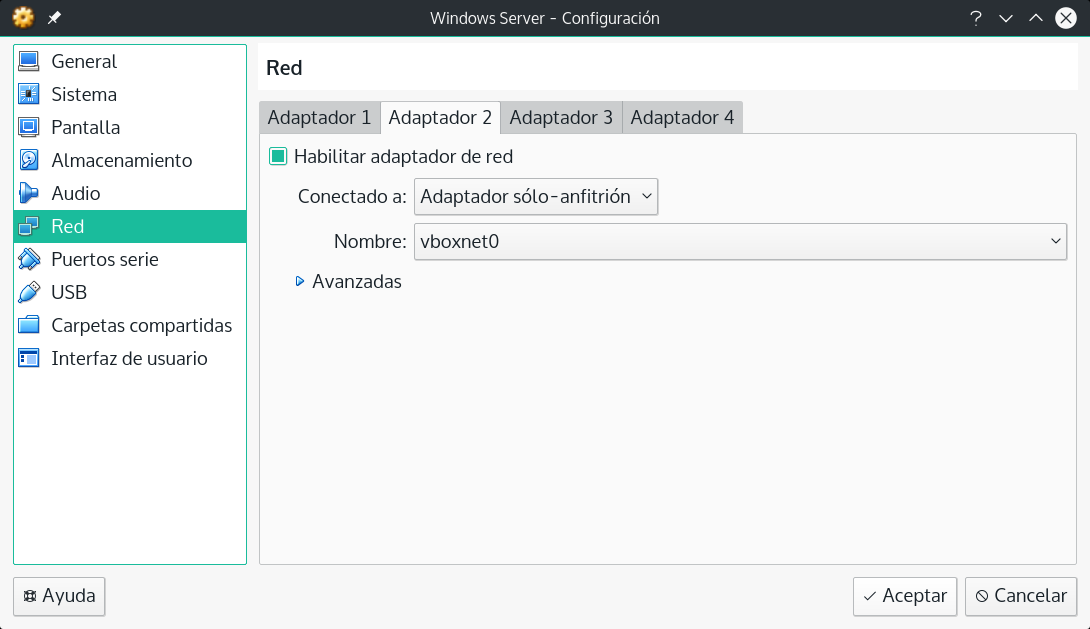
\includegraphics[scale=0.3]{figuras/figura6.png}  %el parámetro scale permite agrandar o achicar la imagen. En el nombre de archivo puede especificar directorios
	\label{figura6}
	
	\caption{Red Host-Only} 
\end{figure}

Ya que la he configurado, y me la ha cogido, tengo que asignarle una dirección IP
\begin{figure}[H] %con el [H] le obligamos a situar aquí la figura
	\centering
	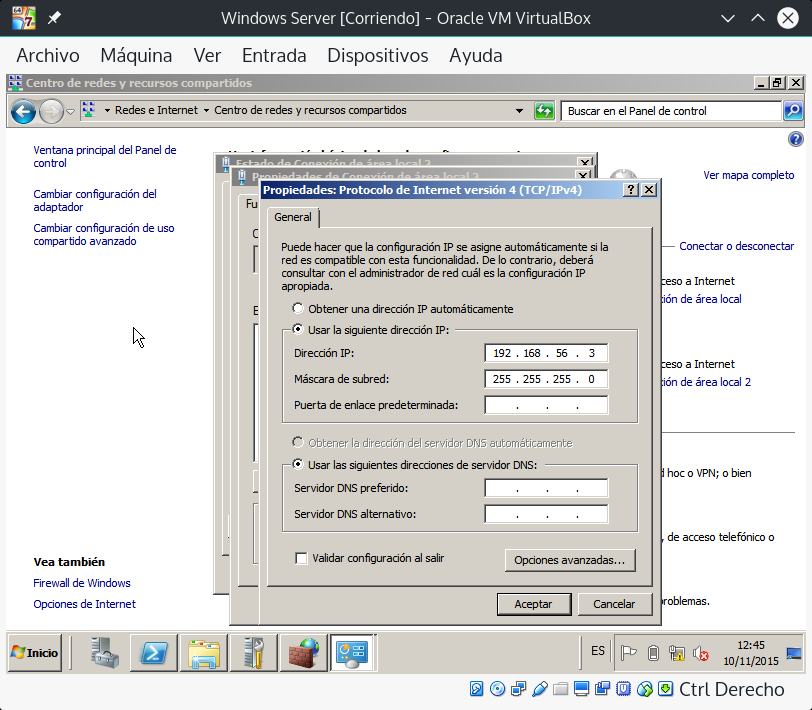
\includegraphics[scale=0.3]{figuras/figura28.png}  %el parámetro scale permite agrandar o achicar la imagen. En el nombre de archivo puede especificar directorios
	\label{figura28}
	
	\caption{Añadimos la dirección IP 192.168.56.3} 
\end{figure}

\begin{figure}[H] %con el [H] le obligamos a situar aquí la figura
	\centering
	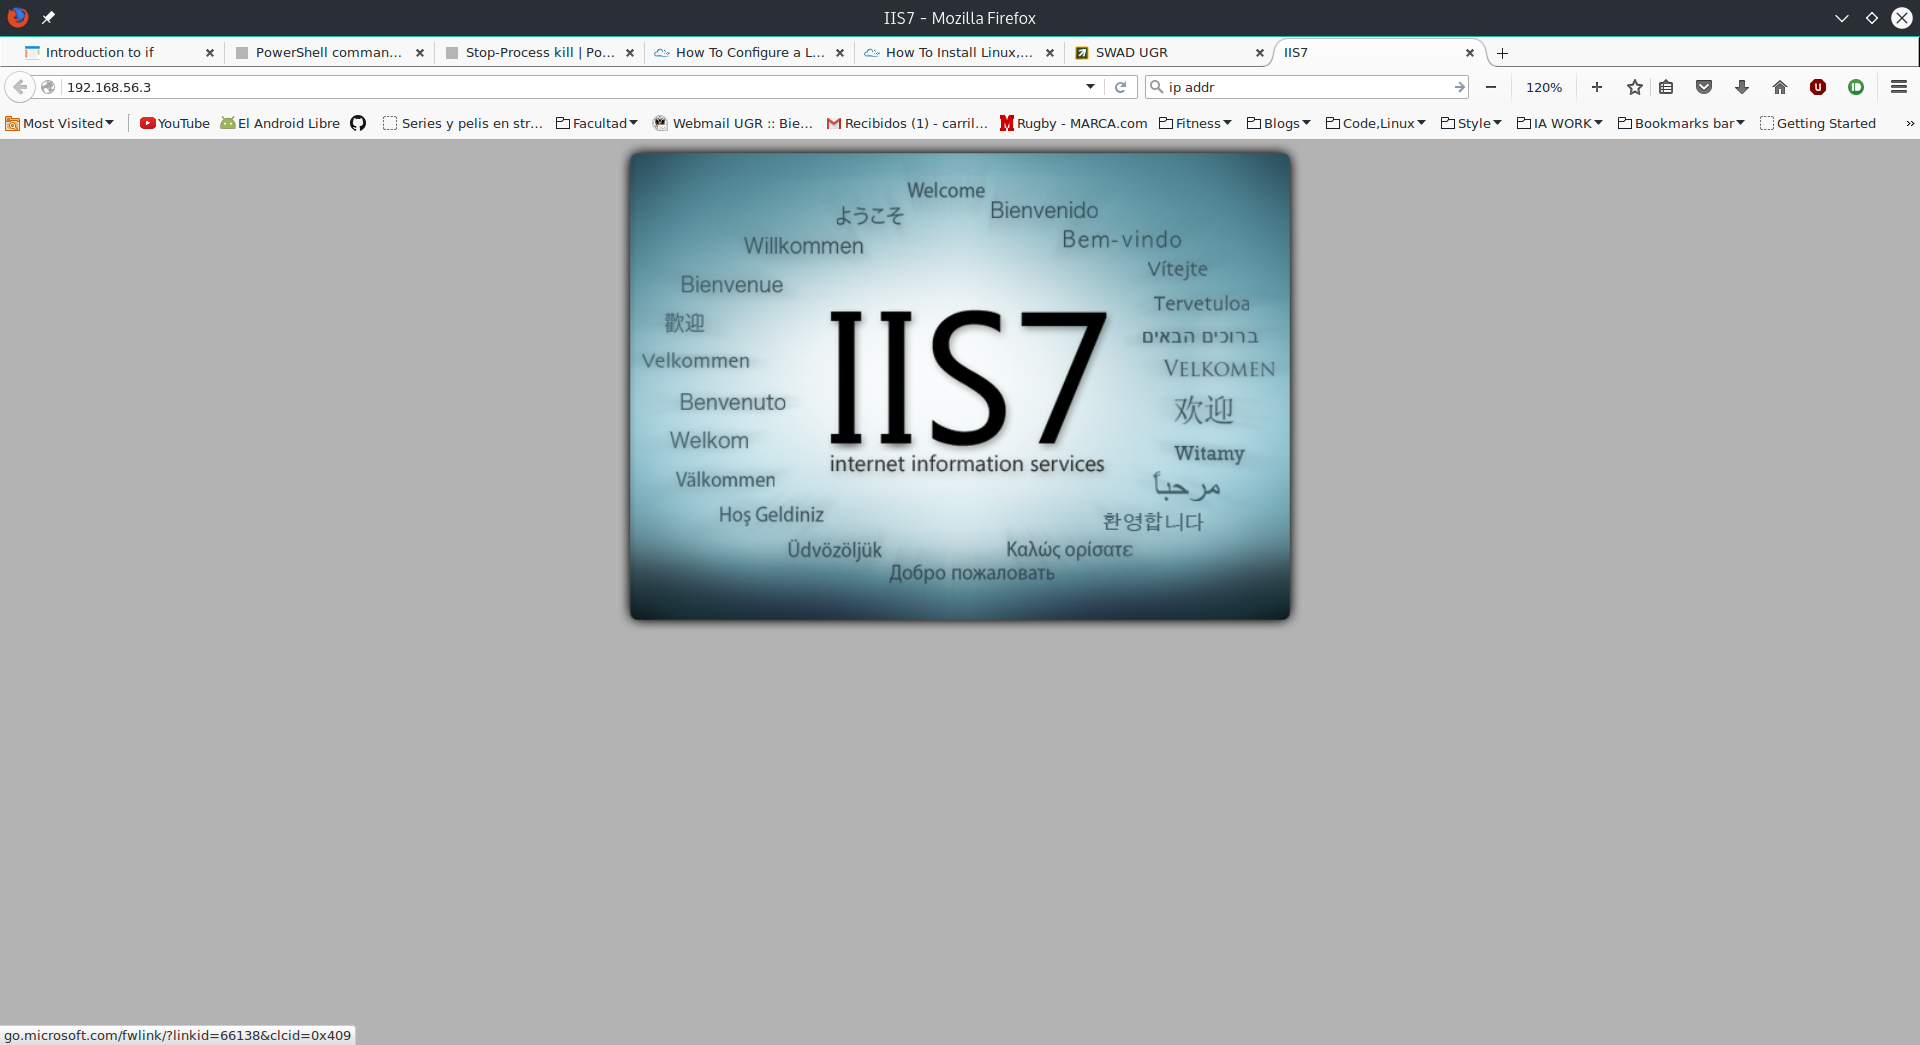
\includegraphics[scale=0.3]{figuras/figura29.png}  %el parámetro scale permite agrandar o achicar la imagen. En el nombre de archivo puede especificar directorios
	\label{figura29}
	
	\caption{Observamos como podemos acceder a la máquina accediendo a la dirección IP} 
\end{figure}
%%%%%%%%%%%%%%%%%%%%%%%%%%%%%%%%%%%%%%%%%%%%%%%%%%%%
% CUESTIÓN 13
%%%%%%%%%%%%%%%%%%%%%%%%%%%%%%%%%%%%%%%%%%%%%%%%%%%%

\section{Cuestión 13: Muestre un ejemplo de uso del comando (p.ej.http://fedoraproject.org/wiki/VMWare)}

Un ejemplo de comando sería:\\
\textbf{patch -p0 -i /tmp/vmware-netfilter.patch} \cite{fedorapatch}
\begin{itemize}
	\item La opción -p0 sirve para dar el nombre entero del archivo sin modificar \cite{patch}
	\item La opción -i nos indica que tiene que leer el parche del pathname que tiene a continuación \cite{patch}
\end{itemize}

%%%%%%%%%%%%%%%%%%%%%%%%%%%%%%%%%%%%%%%%%%%%%%%%%%%%
% CUESTIÓN 14
%%%%%%%%%%%%%%%%%%%%%%%%%%%%%%%%%%%%%%%%%%%%%%%%%%%%

\section{Cuestión 14: Realice la instalación de esta aplicación y pruebe a modificar algún parámetro de algún servicio. Muestre las capturas de pantalla pertinentes así como el proceso de instalación.}

Siguiendo la documentación de DigitalOcean para su instalación \cite{webmin-digital}:
\begin{enumerate}
	\item Primero debemos editar el sources.list para añadir el repositorio para poder instalar webmin con apt-get:\\
	\textbf{sudo vi /etc/apt/sources.list}
	\item Y añadimos estas dos líneas al final del archivo:\\
	\textbf{deb http://download.webmin.com/download/repository sarge contrib}\\
	\textbf{deb http://webmin.mirror.somersettechsolutions.co.uk/repository sarge contrib}
	\item Ahora necesitamos añadir la Webmin GPG key a apt con el comando \ref{figura7}:\\
	\textbf{wget -q http://www.webmin.com/jcameron-key.asc -O- | sudo apt-key add -}
	\begin{figure}[H] %con el [H] le obligamos a situar aquí la figura
		\centering
		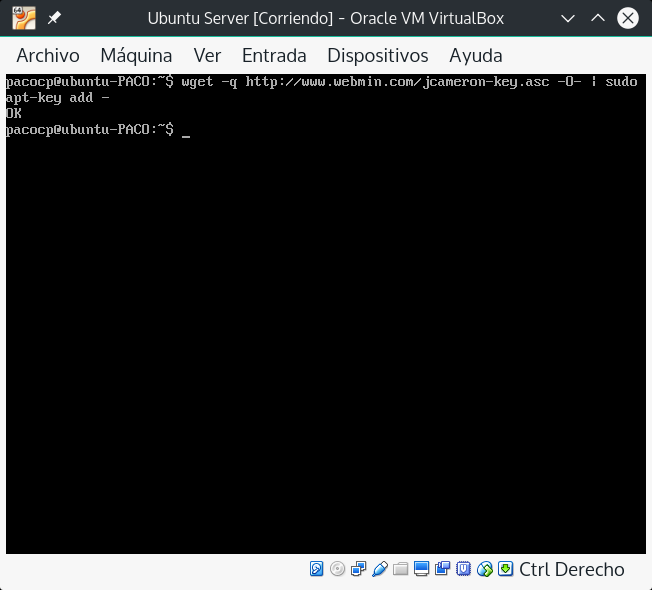
\includegraphics[scale=0.5]{figuras/figura7.png}  %el parámetro scale permite agrandar o achicar la imagen. En el nombre de archivo puede especificar directorios
		\label{figura7}
		
		\caption{Como podemos observar nos pone OK} 
	\end{figure}
	\item Ahora hacemos un update para actualizar los repositorios y la instalación con apt:\\
	\textbf{sudo apt-get update}\\
	\textbf{sudo apt-get install webmin}
	\item Ahora vamos a conectarnos a su servicio, en el puerto 1000:\\
	\textbf{https://192.168.56.2:10000/}
	\begin{figure}[H] %con el [H] le obligamos a situar aquí la figura
		\centering
		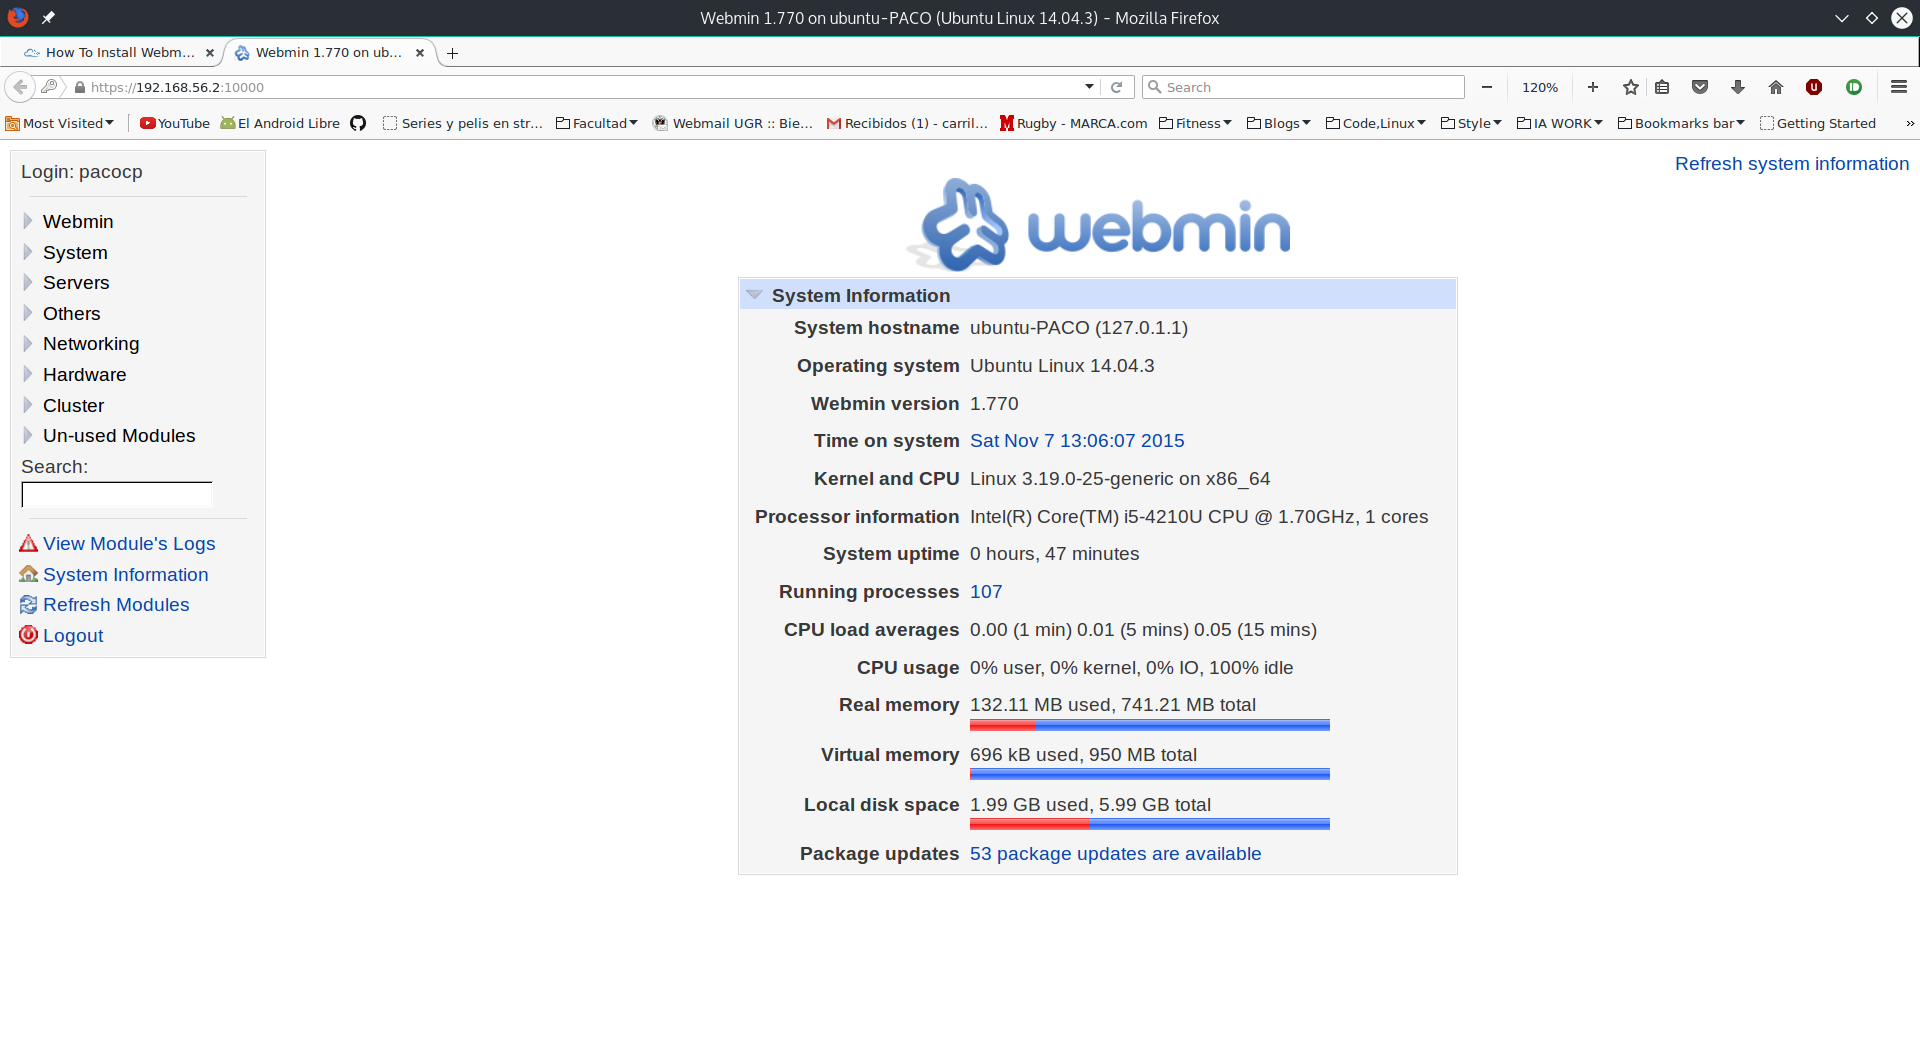
\includegraphics[scale=0.3]{figuras/figura8.png}  %el parámetro scale permite agrandar o achicar la imagen. En el nombre de archivo puede especificar directorios
		\label{figura8}
		
		\caption{Interfaz de webmin} 
	\end{figure}
	
\end{enumerate}
Podemos realizar múltiples actividades desde el menú que se muestra a la izquierda. Una que me ha parecido interesante es la posibilidad de actualizar los paquetes directamente desde aquí:
\begin{figure}[H] %con el [H] le obligamos a situar aquí la figura
	\centering
	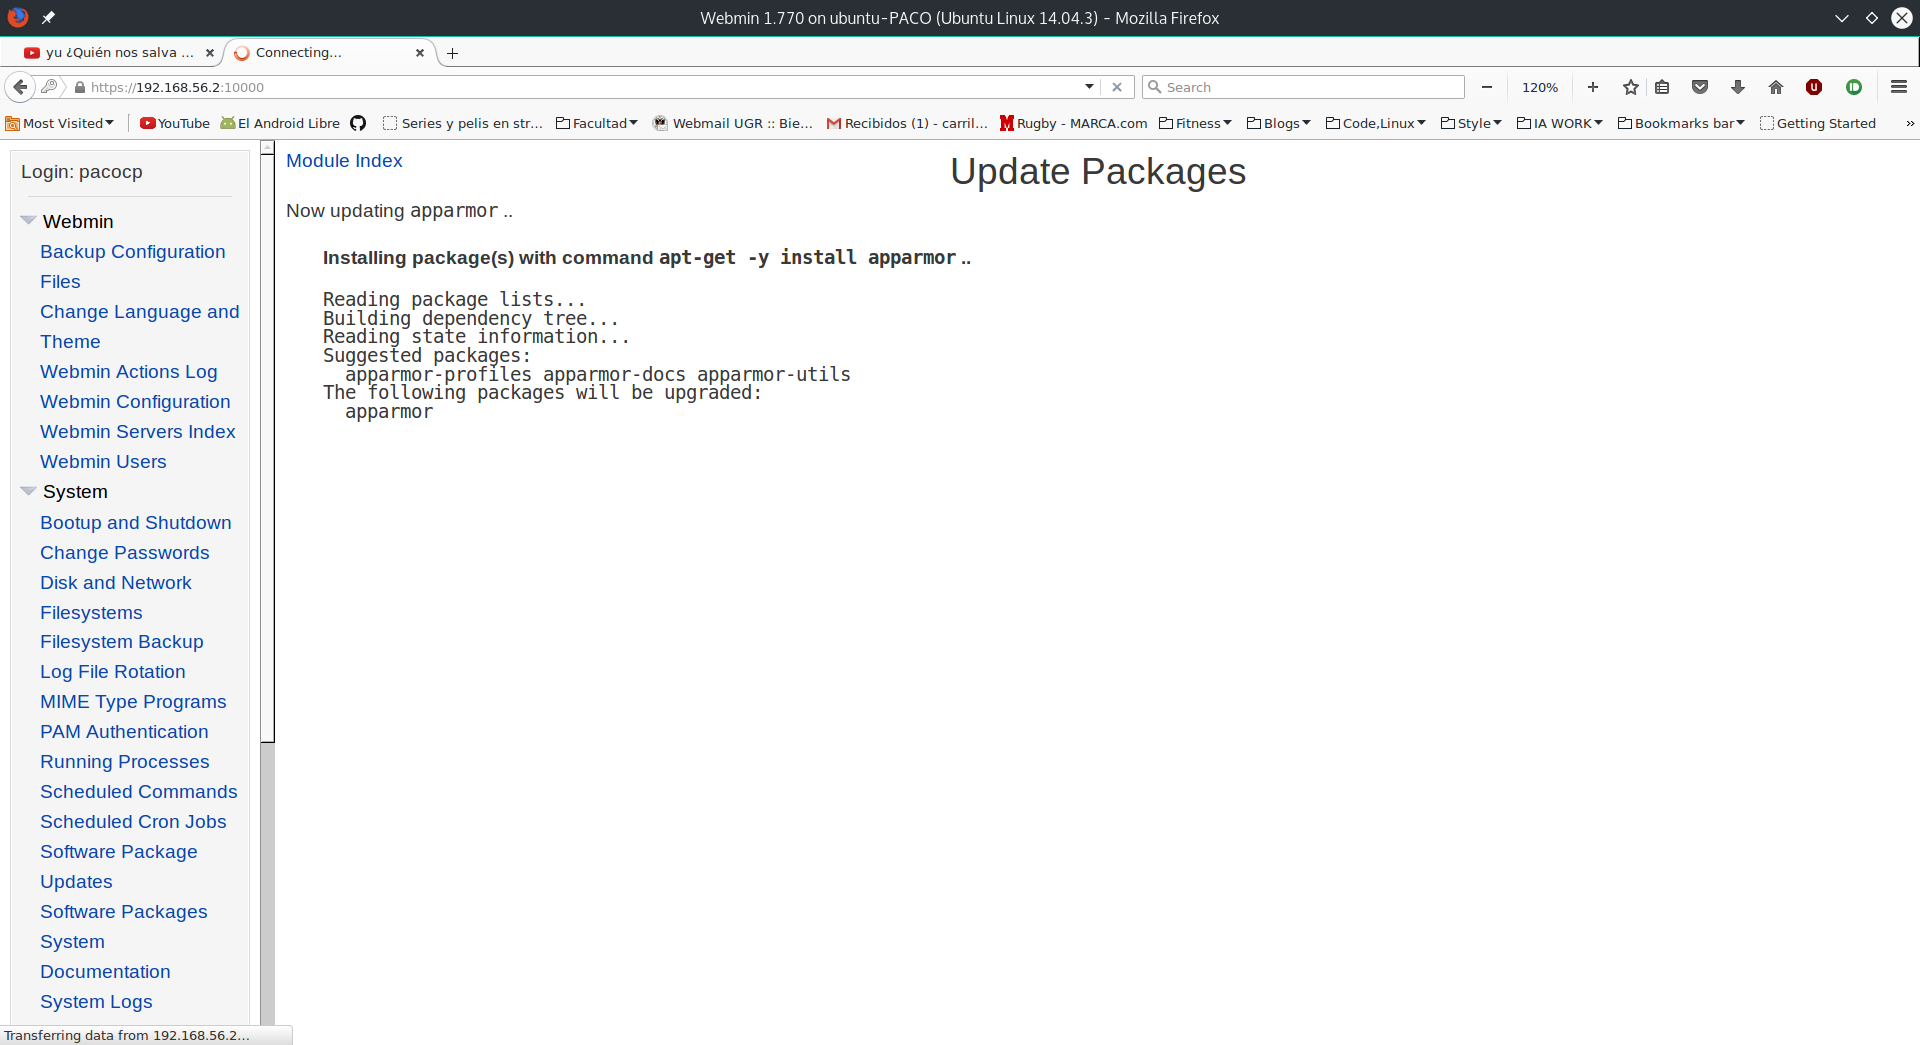
\includegraphics[scale=0.3]{figuras/figura9.png}  %el parámetro scale permite agrandar o achicar la imagen. En el nombre de archivo puede especificar directorios
	\label{figura9}
	
	\caption{Actualizando los paquetes desde Webmin} 
\end{figure}

%%%%%%%%%%%%%%%%%%%%%%%%%%%%%%%%%%%%%%%%%%%%%%%%%%%%
% CUESTIÓN 15
%%%%%%%%%%%%%%%%%%%%%%%%%%%%%%%%%%%%%%%%%%%%%%%%%%%%
\section{Cuestión 15: Instale phpMyAdmin, indique cómo lo ha realizado y muestre algunas capturas de pantalla.Configure PHP para poder importar BDs mayores de 8MiB (límite por defecto). Indique cómo ha realizado el proceso y muestre capturas de pantalla.}
\label{cuestion15}
Siguiendo la documentación de Ubuntu \cite{phpmyadmin}:
\begin{enumerate}
	\item Instalamos phpMyAdmin con el comando: \textbf{sudo apt-get install phpmyadmin}
	\item Una vez que lo hemos instalado modificamos el archivo /etc/apache2/apache2.conf y añadimos la línea:\\
	\textbf{Include /etc/phpmyadmin/apache.conf}\\
	\begin{figure}[H] %con el [H] le obligamos a situar aquí la figura
		\centering
		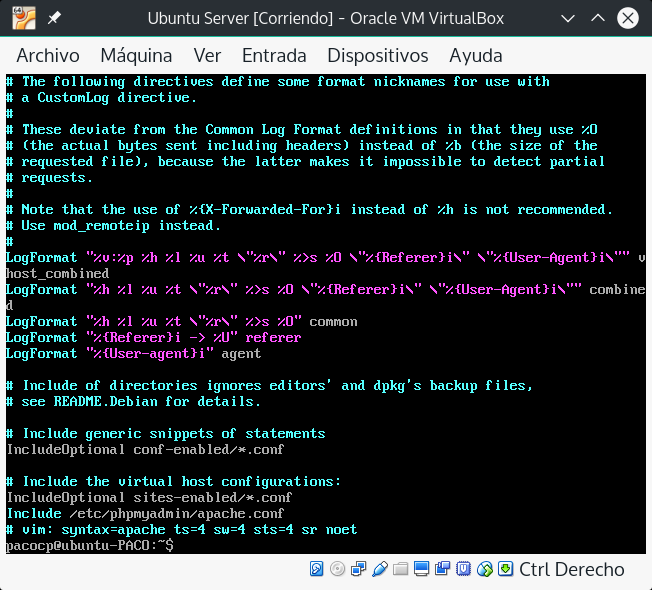
\includegraphics[scale=0.5]{figuras/figura10.png}  %el parámetro scale permite agrandar o achicar la imagen. En el nombre de archivo puede especificar directorios
		\label{figura10}
		
		\caption{Añadiendo la línea al archivo /etc/apache2/apache2.conf} 
	\end{figure}
\end{enumerate}
Ahora ya podemos conectarnos accediendo a la dirección http://192.168.56.2/phpmyadmin . Pero podemos observar que nos da el siguiente error:
\begin{figure}[H] %con el [H] le obligamos a situar aquí la figura
	\centering
	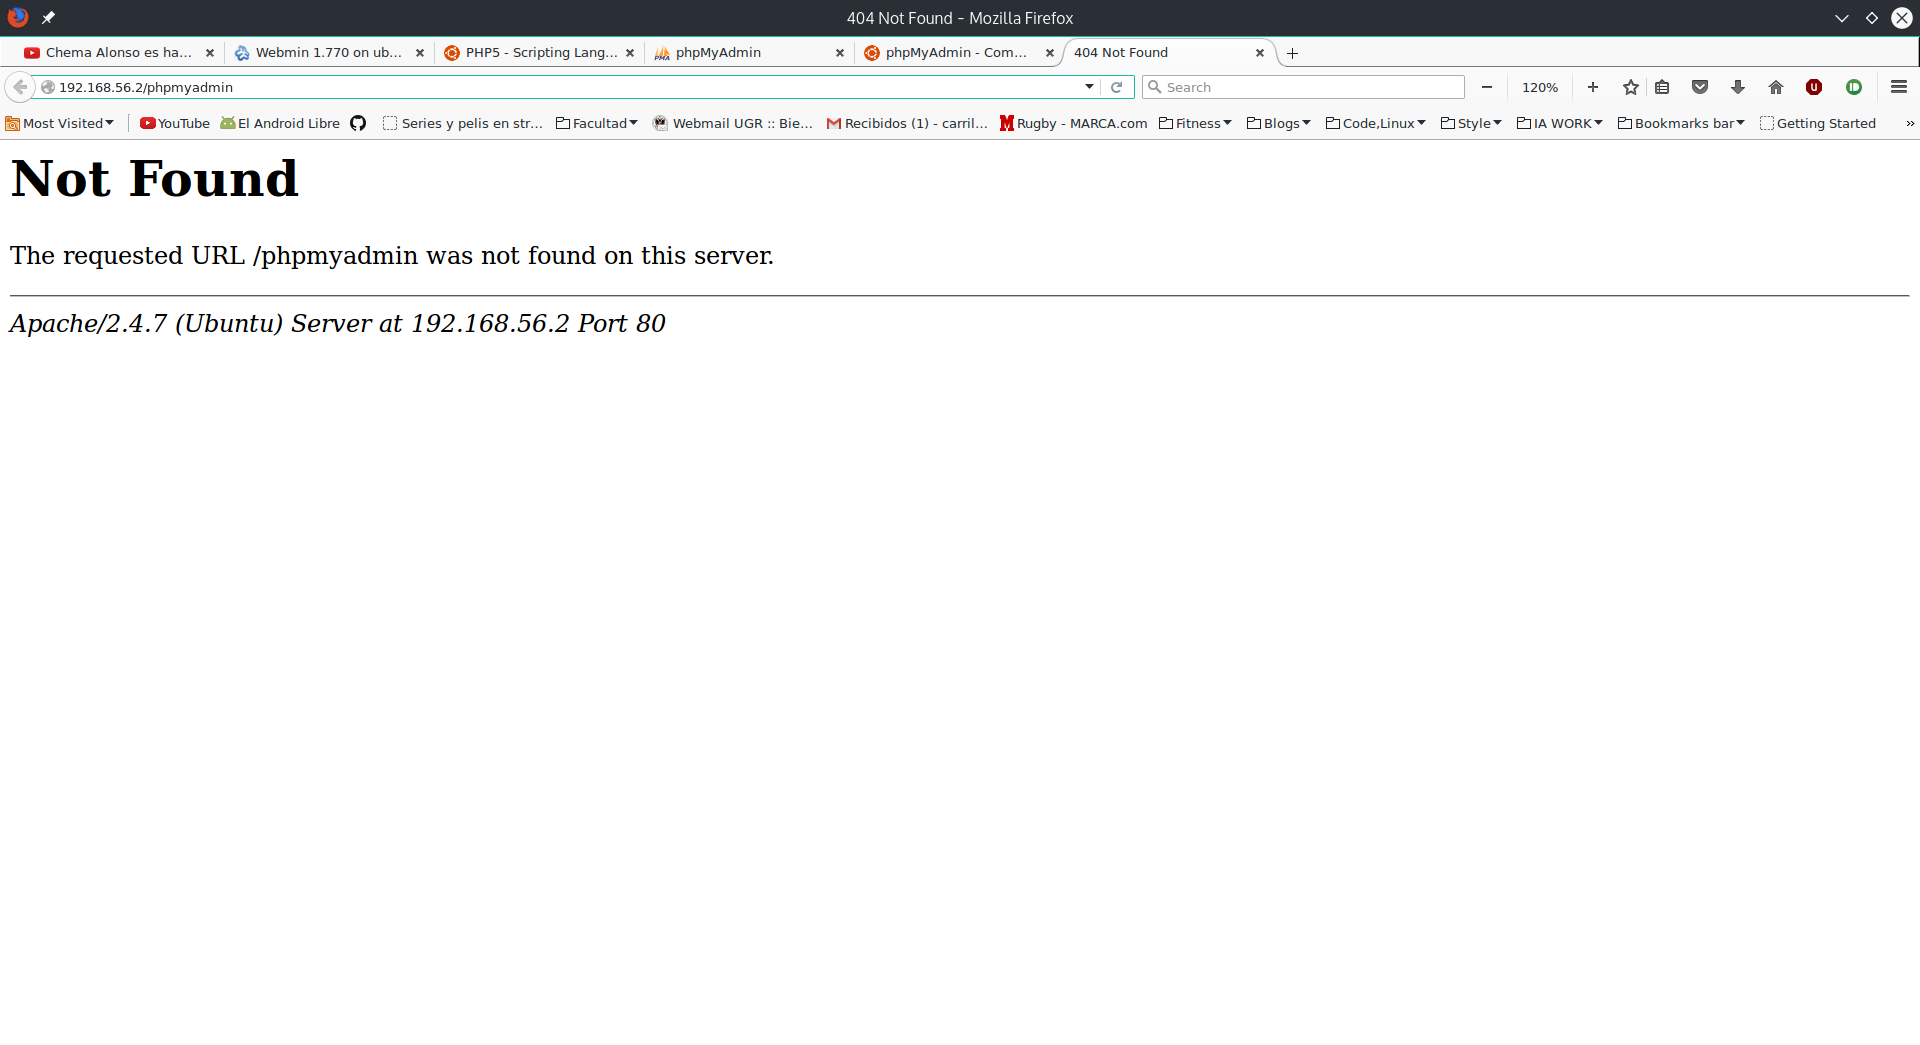
\includegraphics[scale=0.3]{figuras/figura11.png}  %el parámetro scale permite agrandar o achicar la imagen. En el nombre de archivo puede especificar directorios
	\label{figura11}
	
	\caption{Error al intentar acceder} 
\end{figure}
Para poder arreglarlo debemos ejecutar el siguiente comando, para reconfigurar la base de datos, eligiendo Apache 2 cuando se nos da la posibilidad:\\
\textbf{sudo dpkg-reconfigure -plow phpmyadmin}
\begin{figure}[H] %con el [H] le obligamos a situar aquí la figura
	\centering
	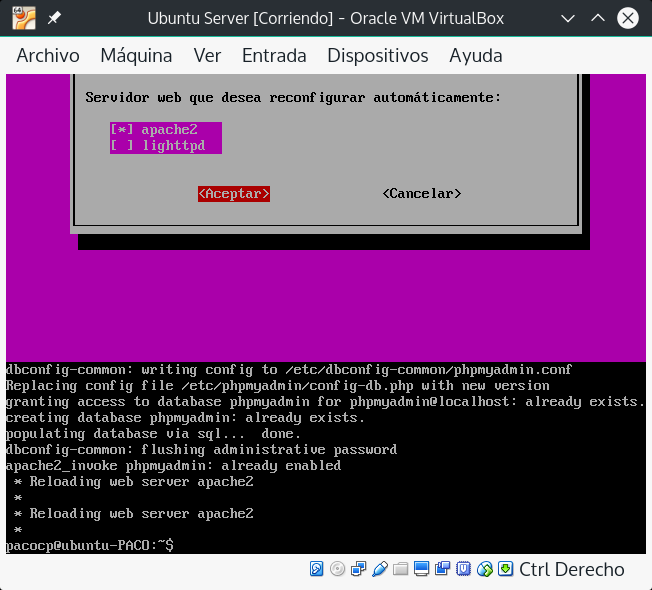
\includegraphics[scale=0.5]{figuras/figura12.png}  %el parámetro scale permite agrandar o achicar la imagen. En el nombre de archivo puede especificar directorios
	\label{figura12}
	
	\caption{Arreglando el error} 
\end{figure}
Y podemos observar como se ha arreglado:
\begin{figure}[H] %con el [H] le obligamos a situar aquí la figura
	\centering
	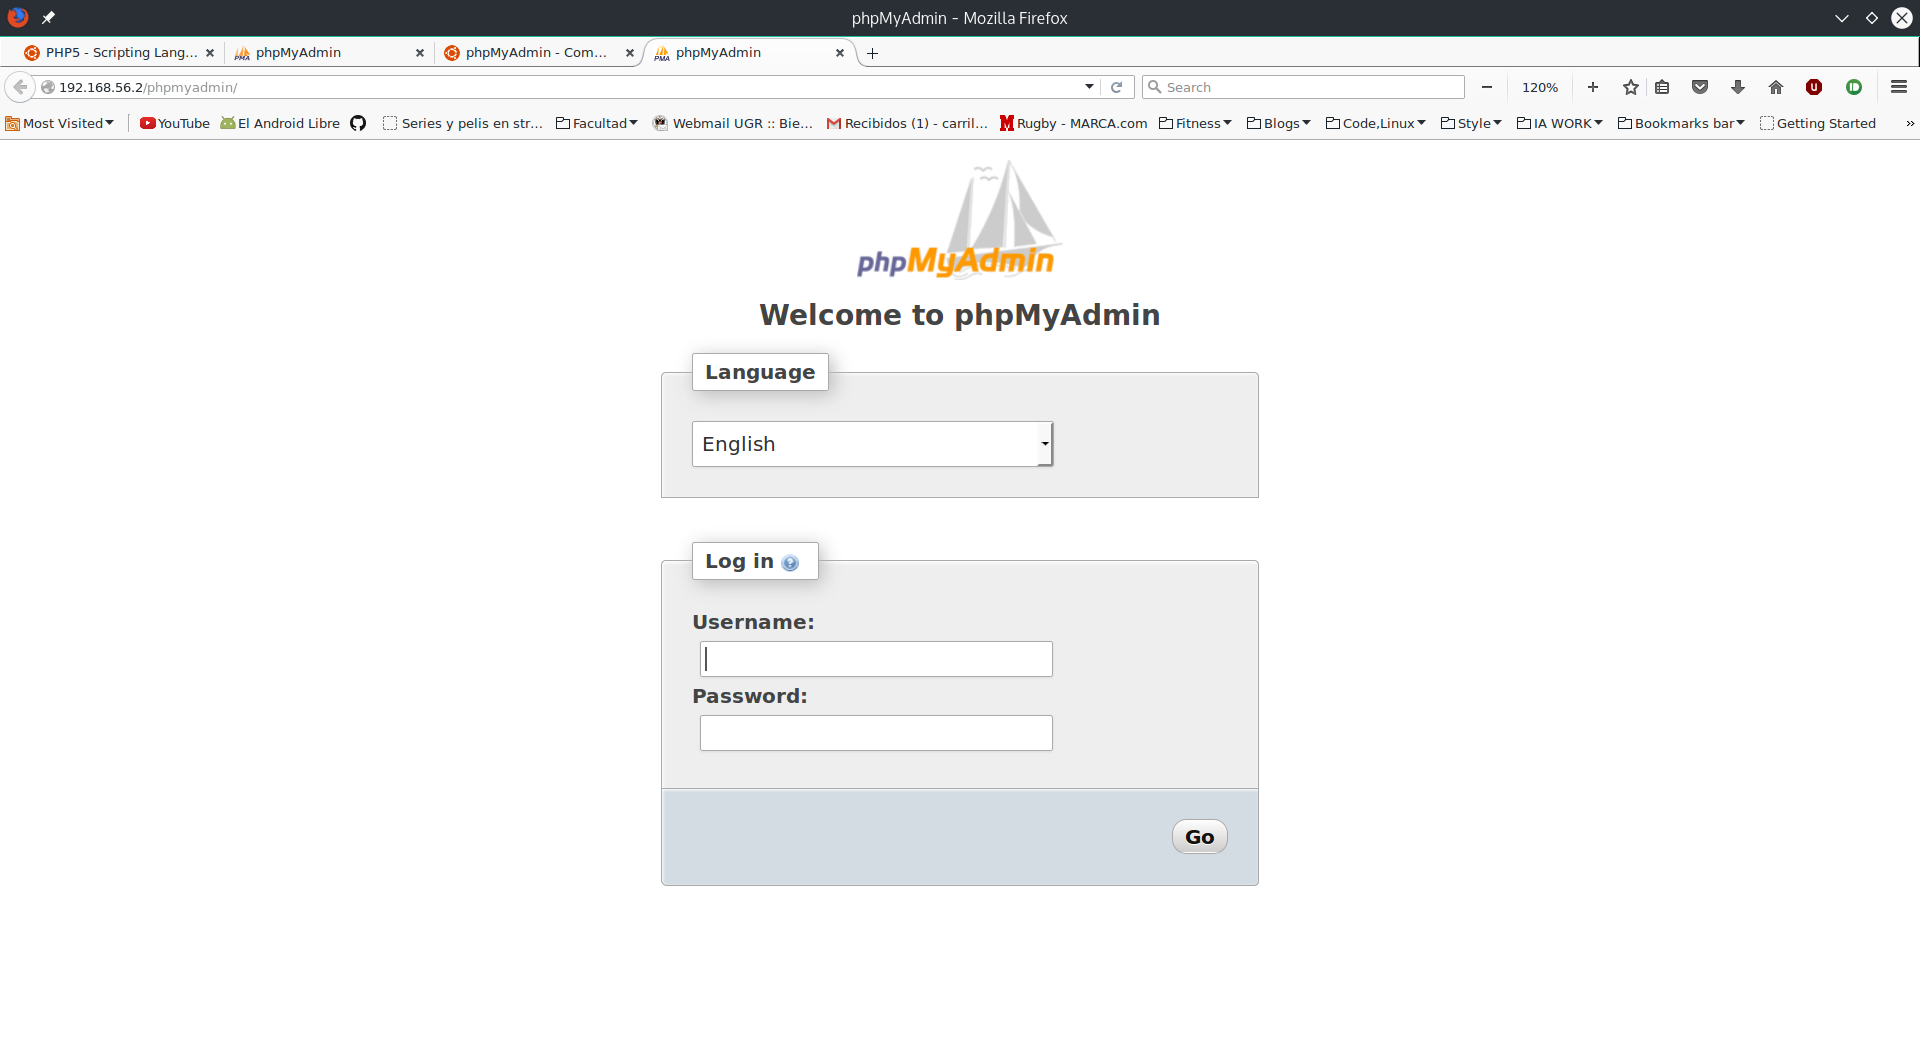
\includegraphics[scale=0.3]{figuras/figura13.png}  %el parámetro scale permite agrandar o achicar la imagen. En el nombre de archivo puede especificar directorios
	\label{figura13}
	
	\caption{Pantalla de inicio de phpMyAdmin} 
\end{figure}
\begin{figure}[H] %con el [H] le obligamos a situar aquí la figura
	\centering
	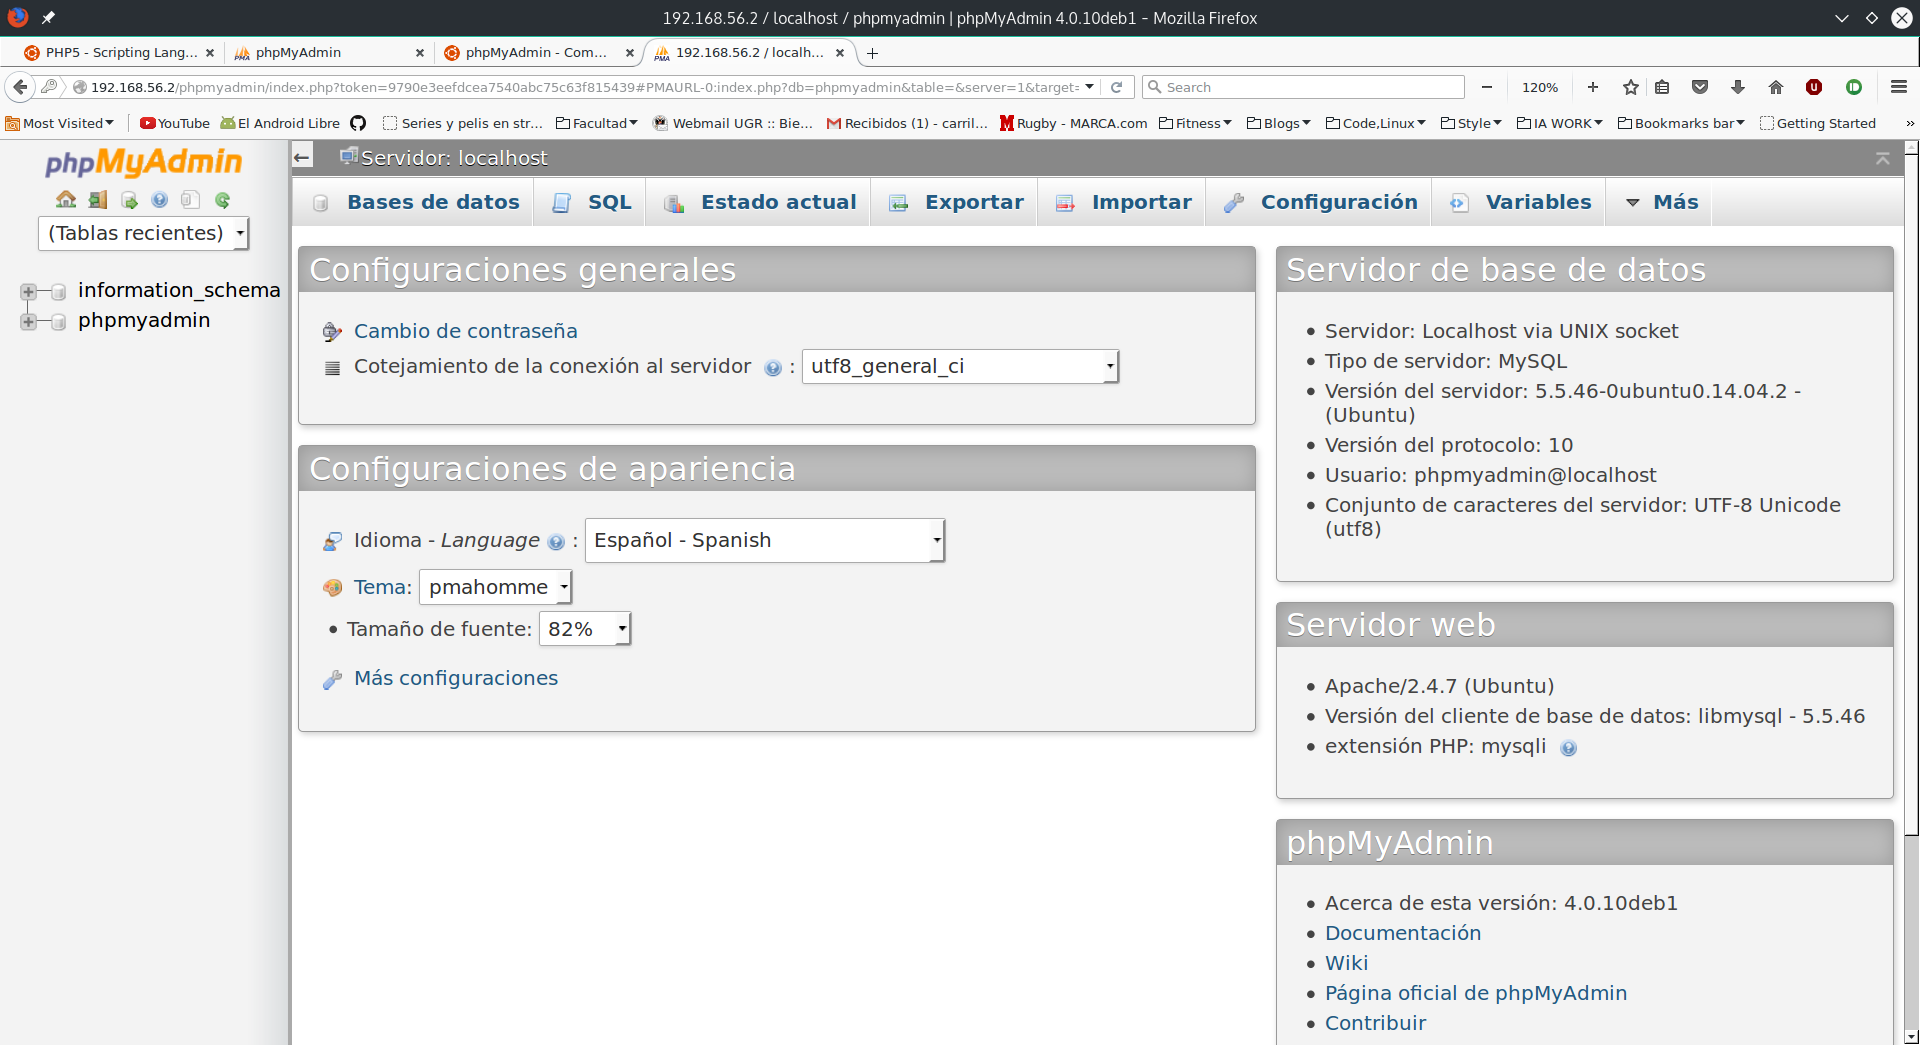
\includegraphics[scale=0.3]{figuras/figura14.png}  %el parámetro scale permite agrandar o achicar la imagen. En el nombre de archivo puede especificar directorios
	\label{figura14}
	
	\caption{Dentro del servicio} 
\end{figure}
 
 Para cambiar el tamaño de las BDs que se pueden importar \cite{php-size} debemos modificar el archivo con el comando \textbf{sudo vi /etc/php5/apache2/php.ini}.
 
\begin{figure}[H] %con el [H] le obligamos a situar aquí la figura
	\centering
	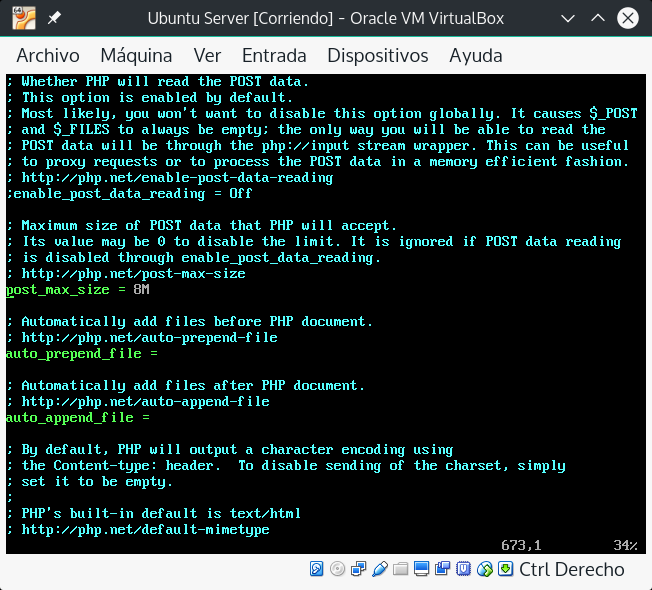
\includegraphics[scale=0.5]{figuras/figura24.png}  %el parámetro scale permite agrandar o achicar la imagen. En el nombre de archivo puede especificar directorios
	\label{figura24}
	
	\caption{Vemos como en la línea post\_max\_size = 8MB , que es el valor por defecto } 
\end{figure}

\begin{figure}[H] %con el [H] le obligamos a situar aquí la figura
	\centering
	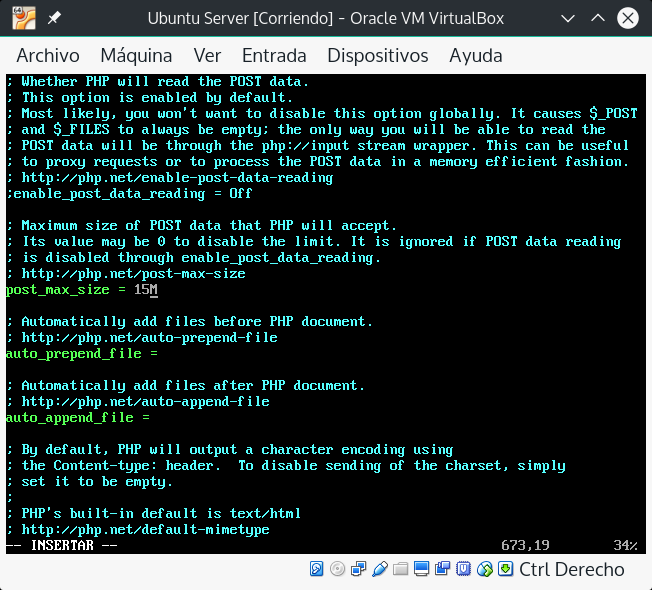
\includegraphics[scale=0.5]{figuras/figura25.png}  %el parámetro scale permite agrandar o achicar la imagen. En el nombre de archivo puede especificar directorios
	\label{figura25}
	
	\caption{Lo cambiamos por  post\_max\_size = 15MB , para que acepte bases de datos de hasta 15MB} 
\end{figure}

También debemos modificar el valor de upload\_max\_filesize al mismo valor que hemos indicado antes, que se encuentra en el mismo archivo que el anterior parámetro.

\begin{figure}[H] %con el [H] le obligamos a situar aquí la figura
	\centering
	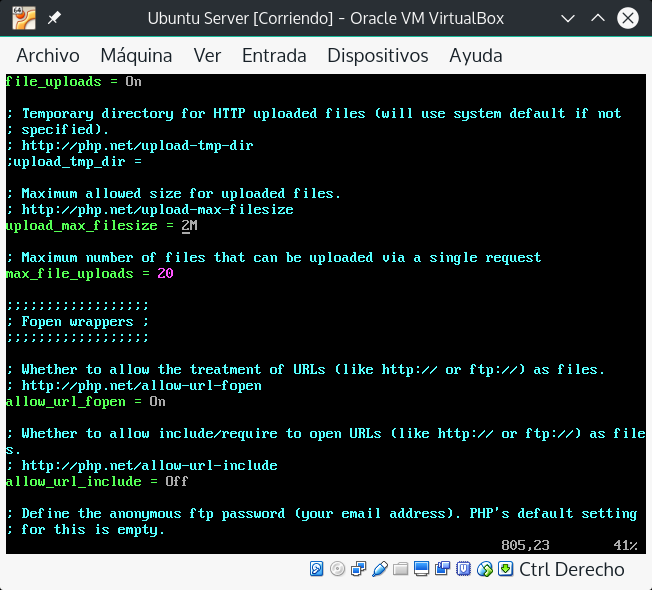
\includegraphics[scale=0.5]{figuras/figura32.png}  %el parámetro scale permite agrandar o achicar la imagen. En el nombre de archivo puede especificar directorios
	\label{figura32}
	
	\caption{Vemos como en la línea  upload\_max\_filesize = 2MB , que es el valor por defecto } 
\end{figure}

\begin{figure}[H] %con el [H] le obligamos a situar aquí la figura
	\centering
	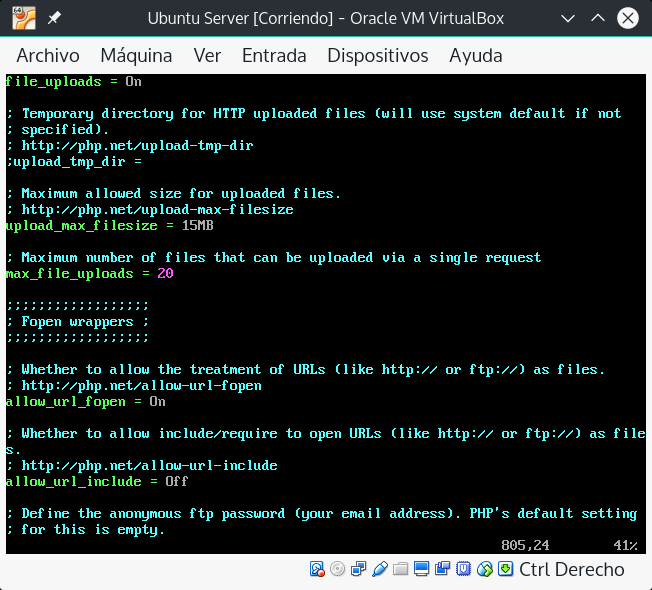
\includegraphics[scale=0.5]{figuras/figura33.png}  %el parámetro scale permite agrandar o achicar la imagen. En el nombre de archivo puede especificar directorios
	\label{figura33}
	
	\caption{Lo cambiamos por  upload\_max\_filesize = 15MB , para que acepte bases de datos de hasta 15MB} 
\end{figure}
Ahora necesitamos reiniciar el servicio de apache para que se apliquen los cambios (lo he supuesto ya que la carpeta donde se encuentra el archivo es apache2):
\textbf{sudo service apache2 restart}\\

Y si ahora nos metemos en phpmyadmin podemos observar que el máximo que nos deja es 15MB.

\begin{figure}[H] %con el [H] le obligamos a situar aquí la figura
	\centering
	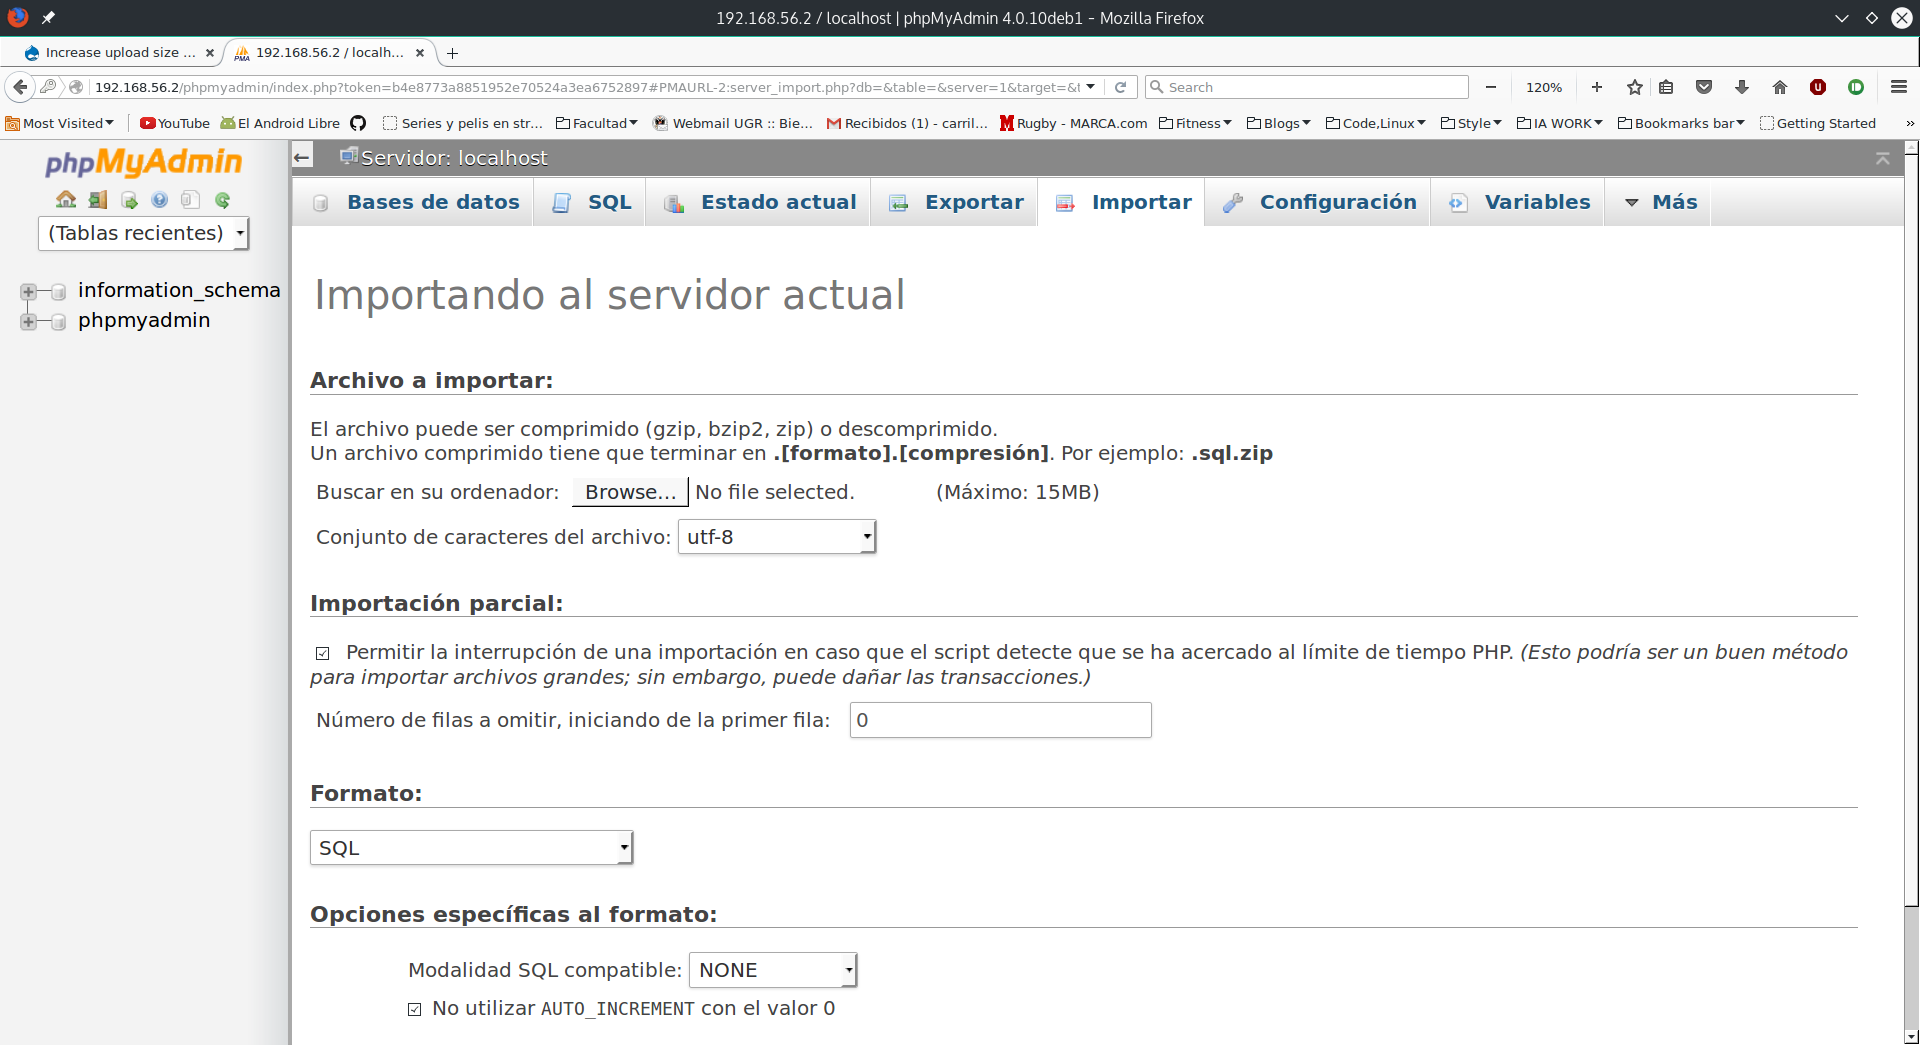
\includegraphics[scale=0.3]{figuras/figura34.png}  %el parámetro scale permite agrandar o achicar la imagen. En el nombre de archivo puede especificar directorios
	\label{figura34}
	
	\caption{Podemos observar como 15MB es lo máximo que nos deja subir} 
\end{figure}
%%%%%%%%%%%%%%%%%%%%%%%%%%%%%%%%%%%%%%%%%%%%%%%%%%%%
% CUESTIÓN 16
%%%%%%%%%%%%%%%%%%%%%%%%%%%%%%%%%%%%%%%%%%%%%%%%%%%%

\section{Cuestión 16: Viste al menos una de las webs de los software mencionados y pruebe las demos que ofrecen realizando capturas de pantalla y comentando qué está realizando.}
Vamos a probar la web de DirectAdmin \cite{directadmin}:\\
\begin{figure}[H] %con el [H] le obligamos a situar aquí la figura
	\centering
	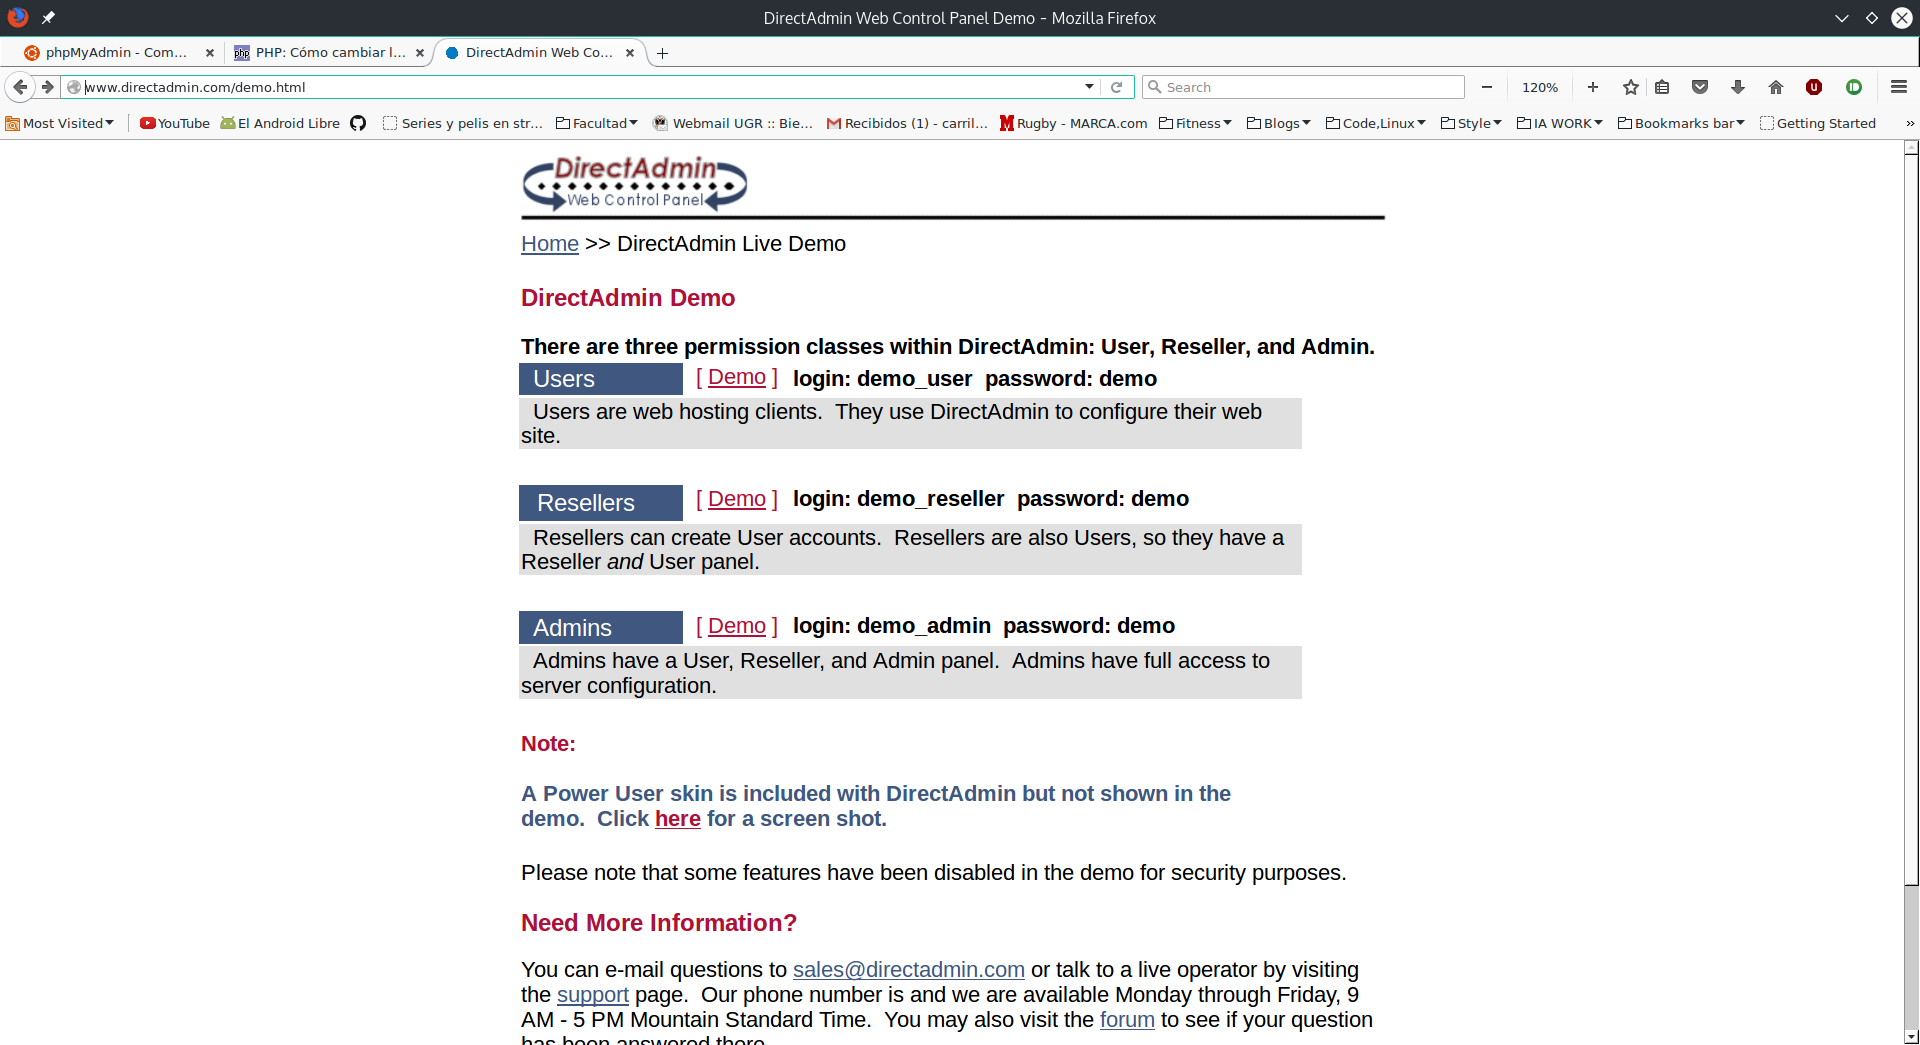
\includegraphics[scale=0.3]{figuras/figura15.png}  %el parámetro scale permite agrandar o achicar la imagen. En el nombre de archivo puede especificar directorios
	\label{figura15}
	
	\caption{Elegimos la opción de admin} 
\end{figure}

\begin{figure}[H] %con el [H] le obligamos a situar aquí la figura
	\centering
	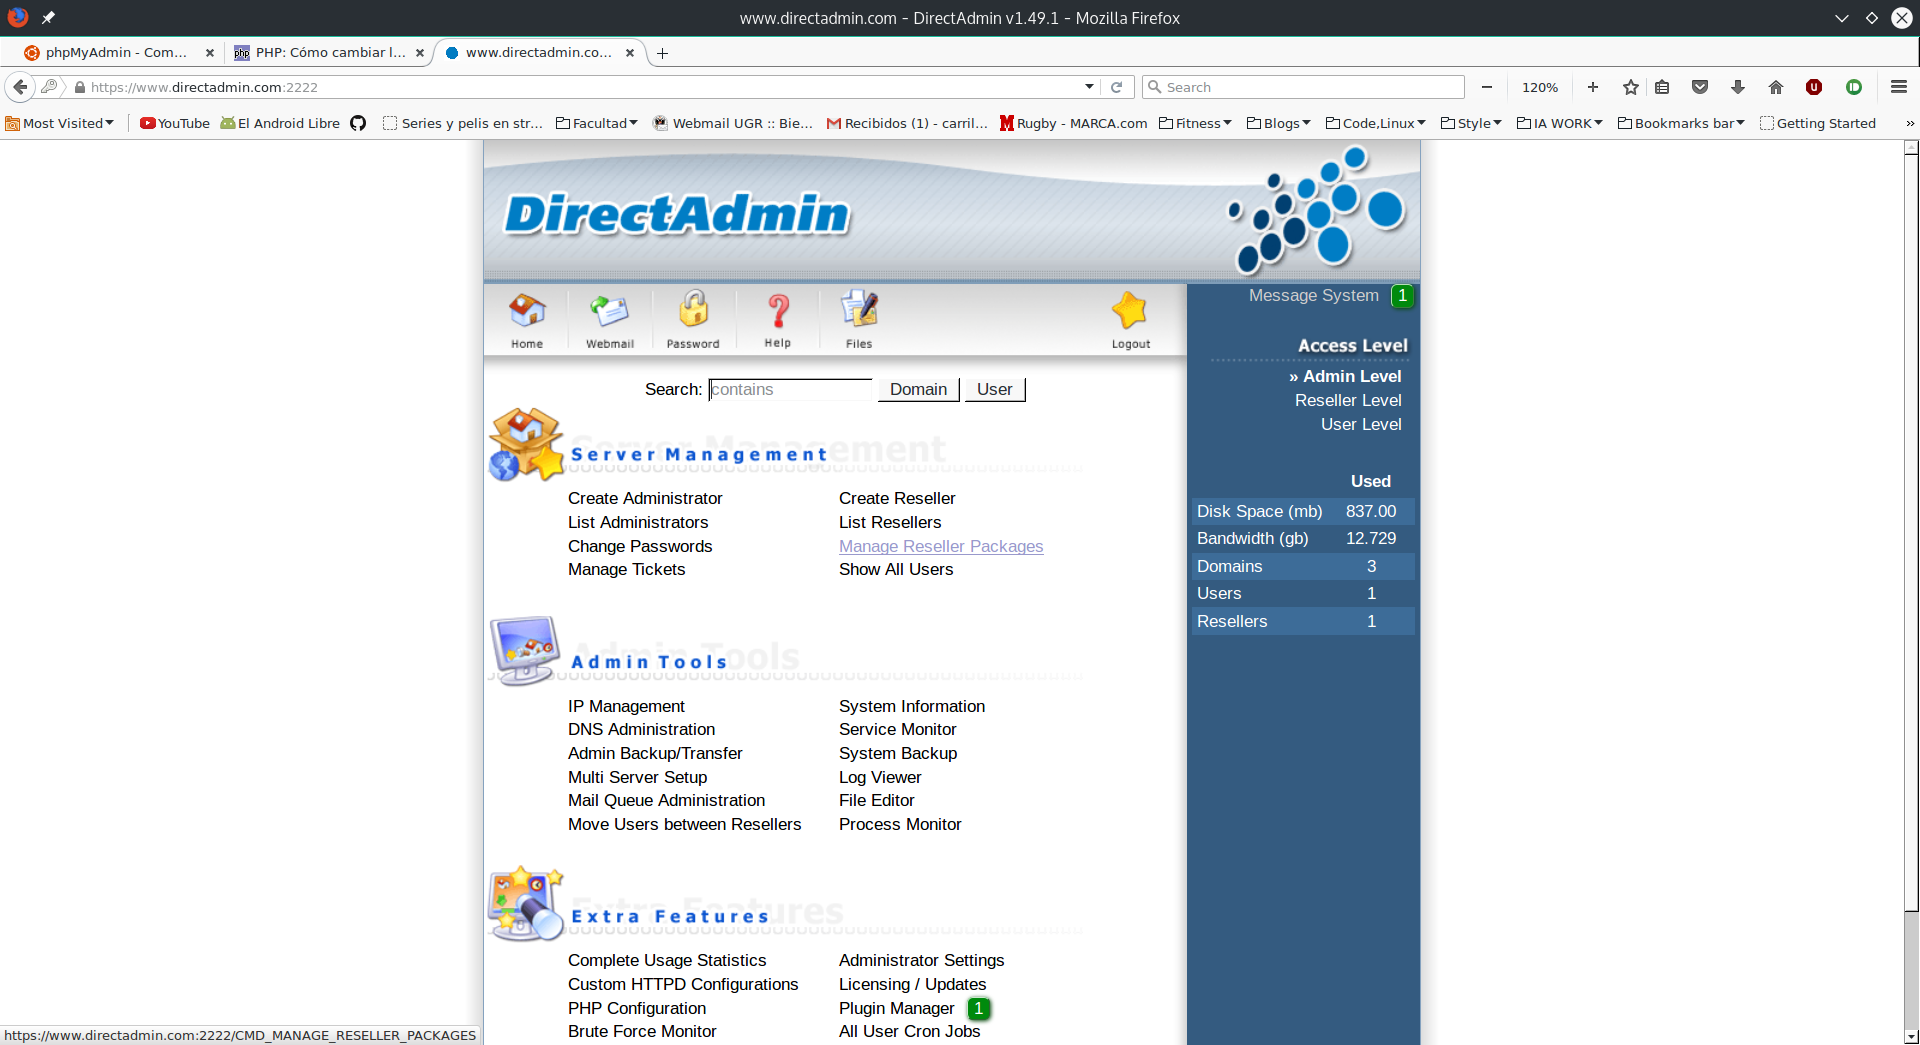
\includegraphics[scale=0.3]{figuras/figura16.png}  %el parámetro scale permite agrandar o achicar la imagen. En el nombre de archivo puede especificar directorios
	\label{figura16}
	
	\caption{Nos encontramos con el panel de control} 
\end{figure}

\begin{figure}[H] %con el [H] le obligamos a situar aquí la figura
	\centering
	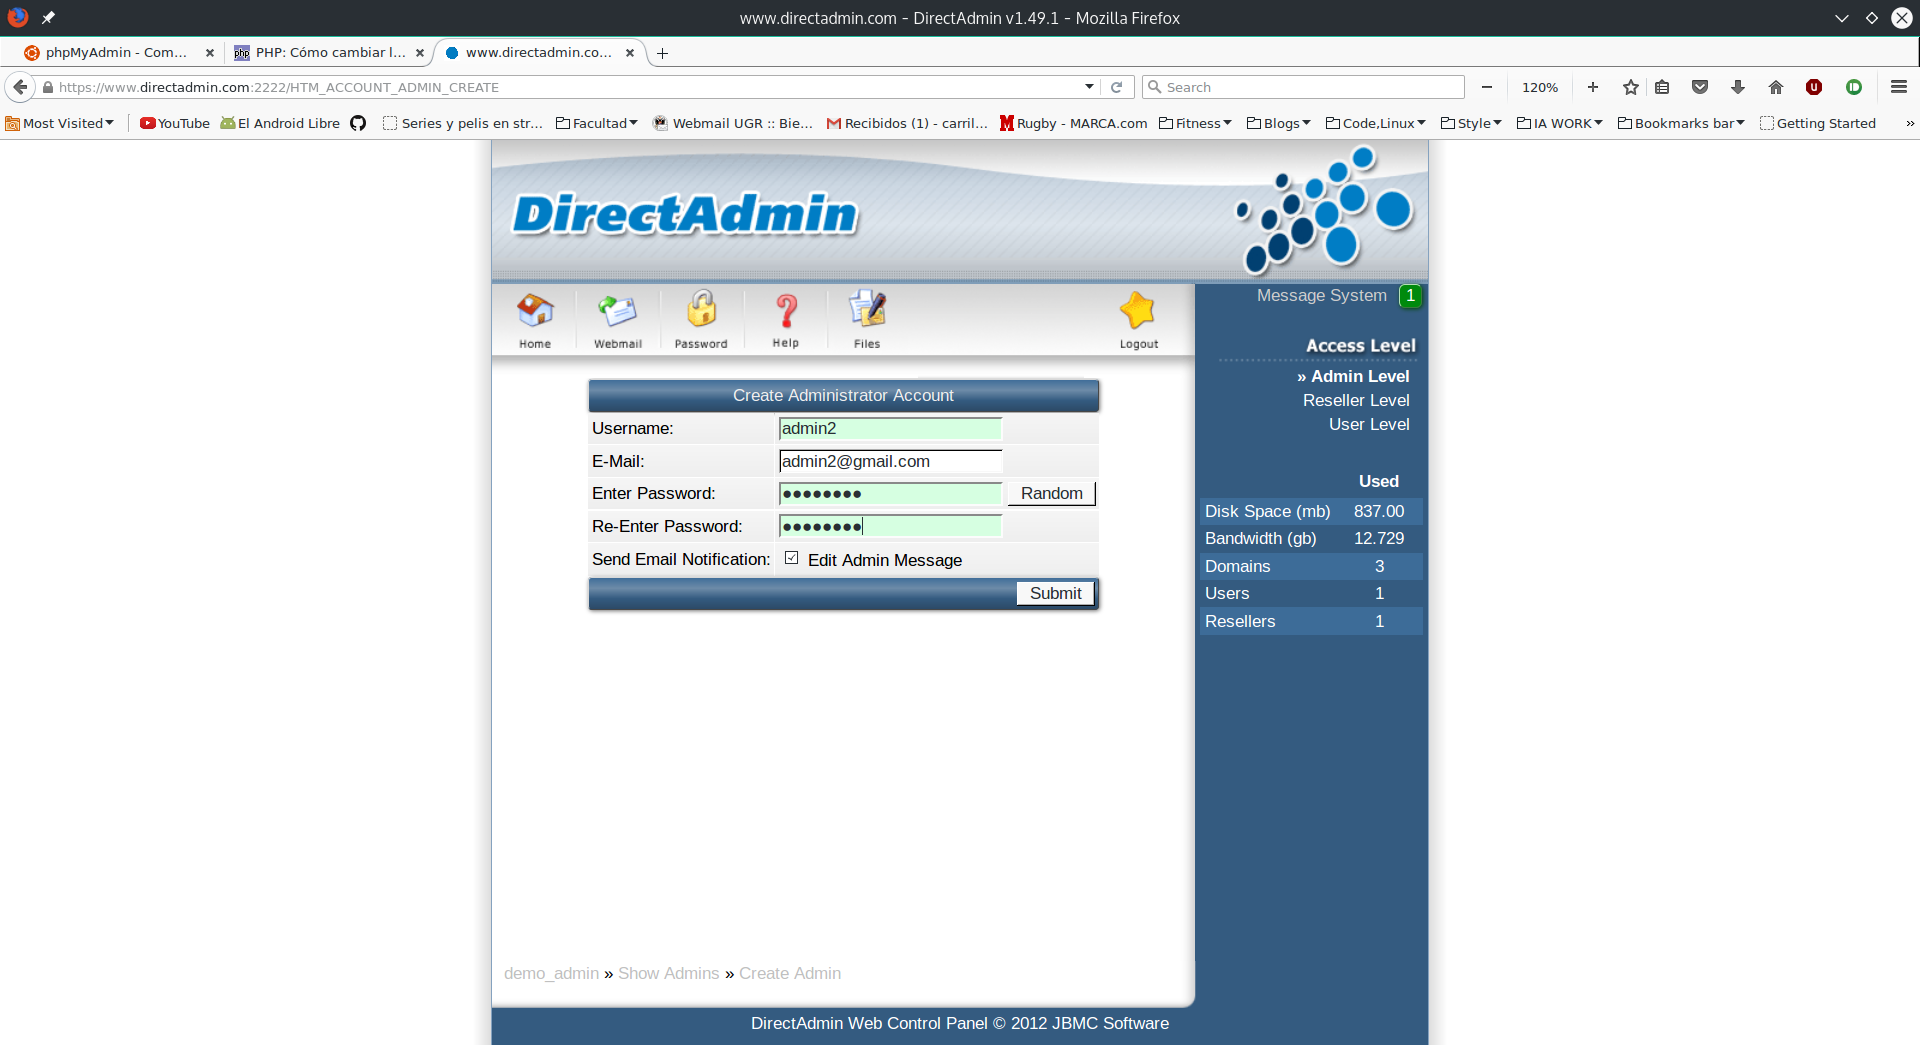
\includegraphics[scale=0.3]{figuras/figura17.png}  %el parámetro scale permite agrandar o achicar la imagen. En el nombre de archivo puede especificar directorios
	\label{figura17}
	
	\caption{Podemos crear nuevos administradores} 
\end{figure}

\begin{figure}[H] %con el [H] le obligamos a situar aquí la figura
	\centering
	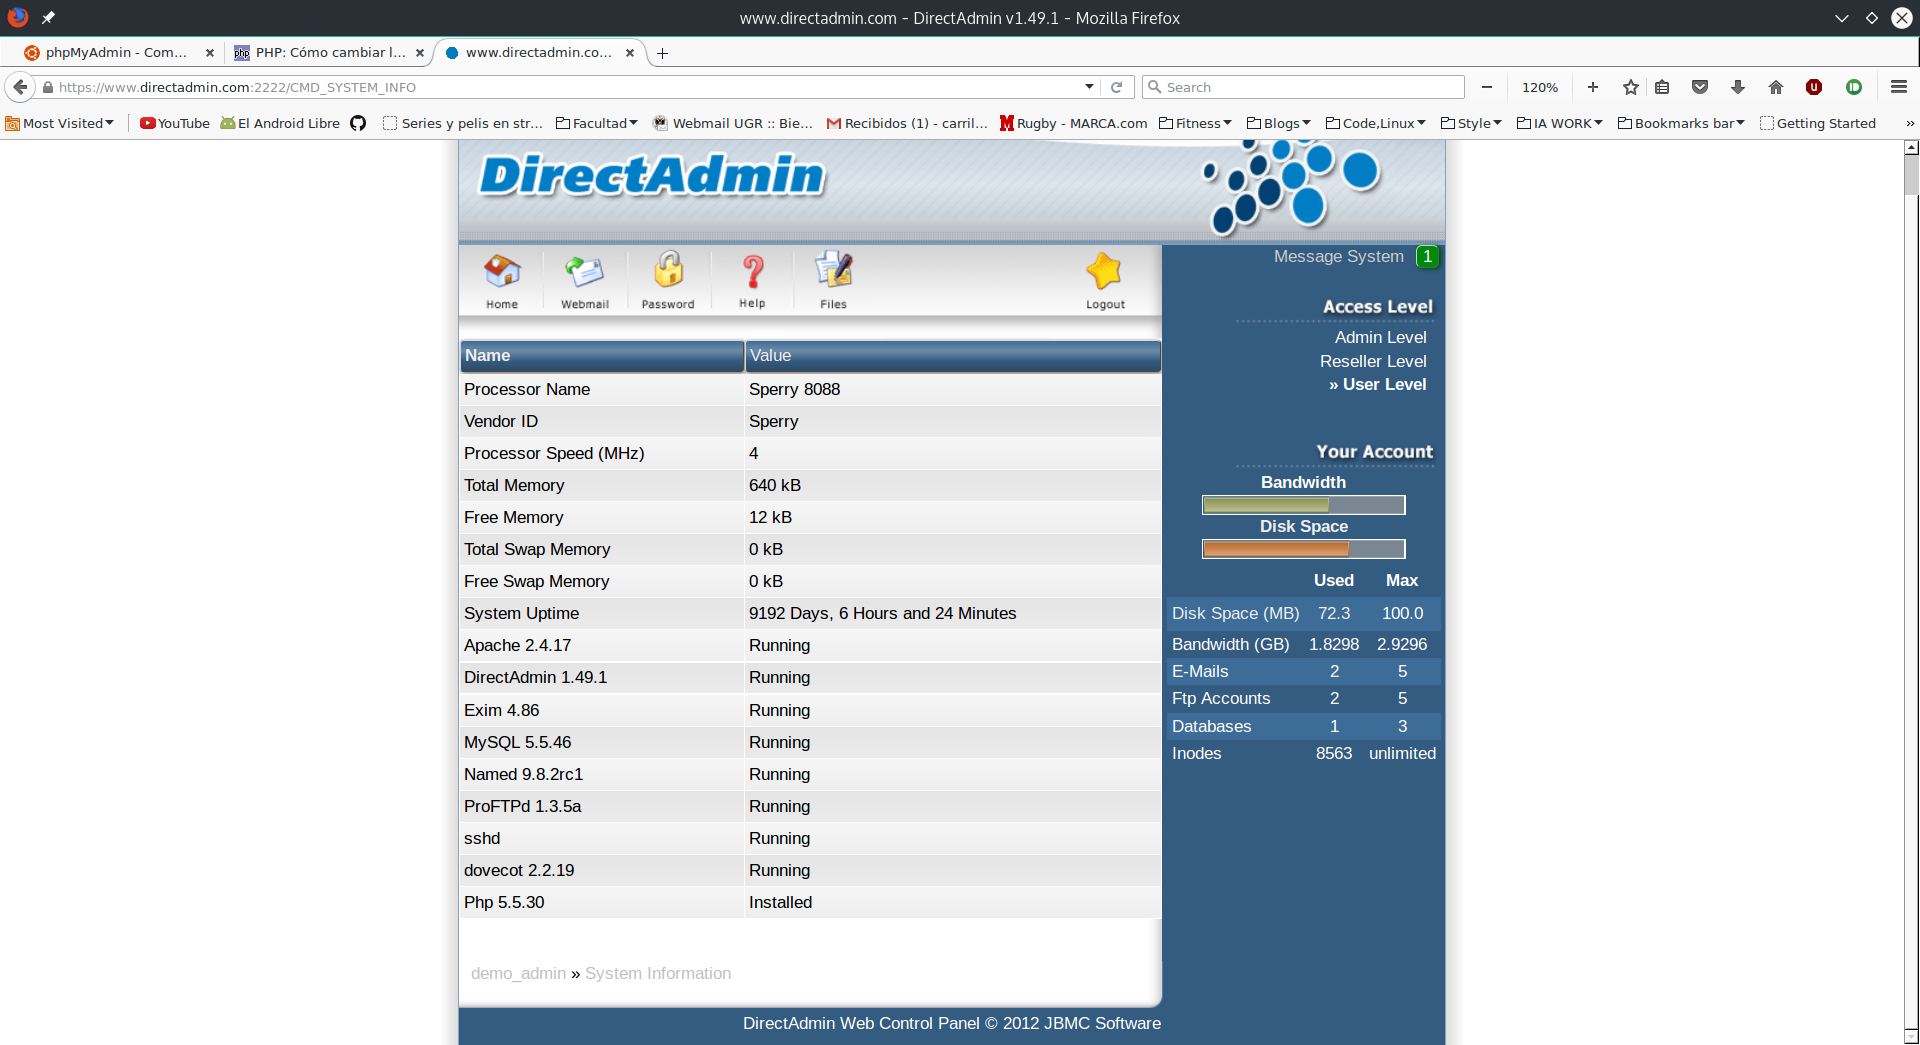
\includegraphics[scale=0.3]{figuras/figura18.png}  %el parámetro scale permite agrandar o achicar la imagen. En el nombre de archivo puede especificar directorios
	\label{figura18}
	
	\caption{O ver la información del sistema, algo muy útil} 
\end{figure}

\begin{figure}[H] %con el [H] le obligamos a situar aquí la figura
	\centering
	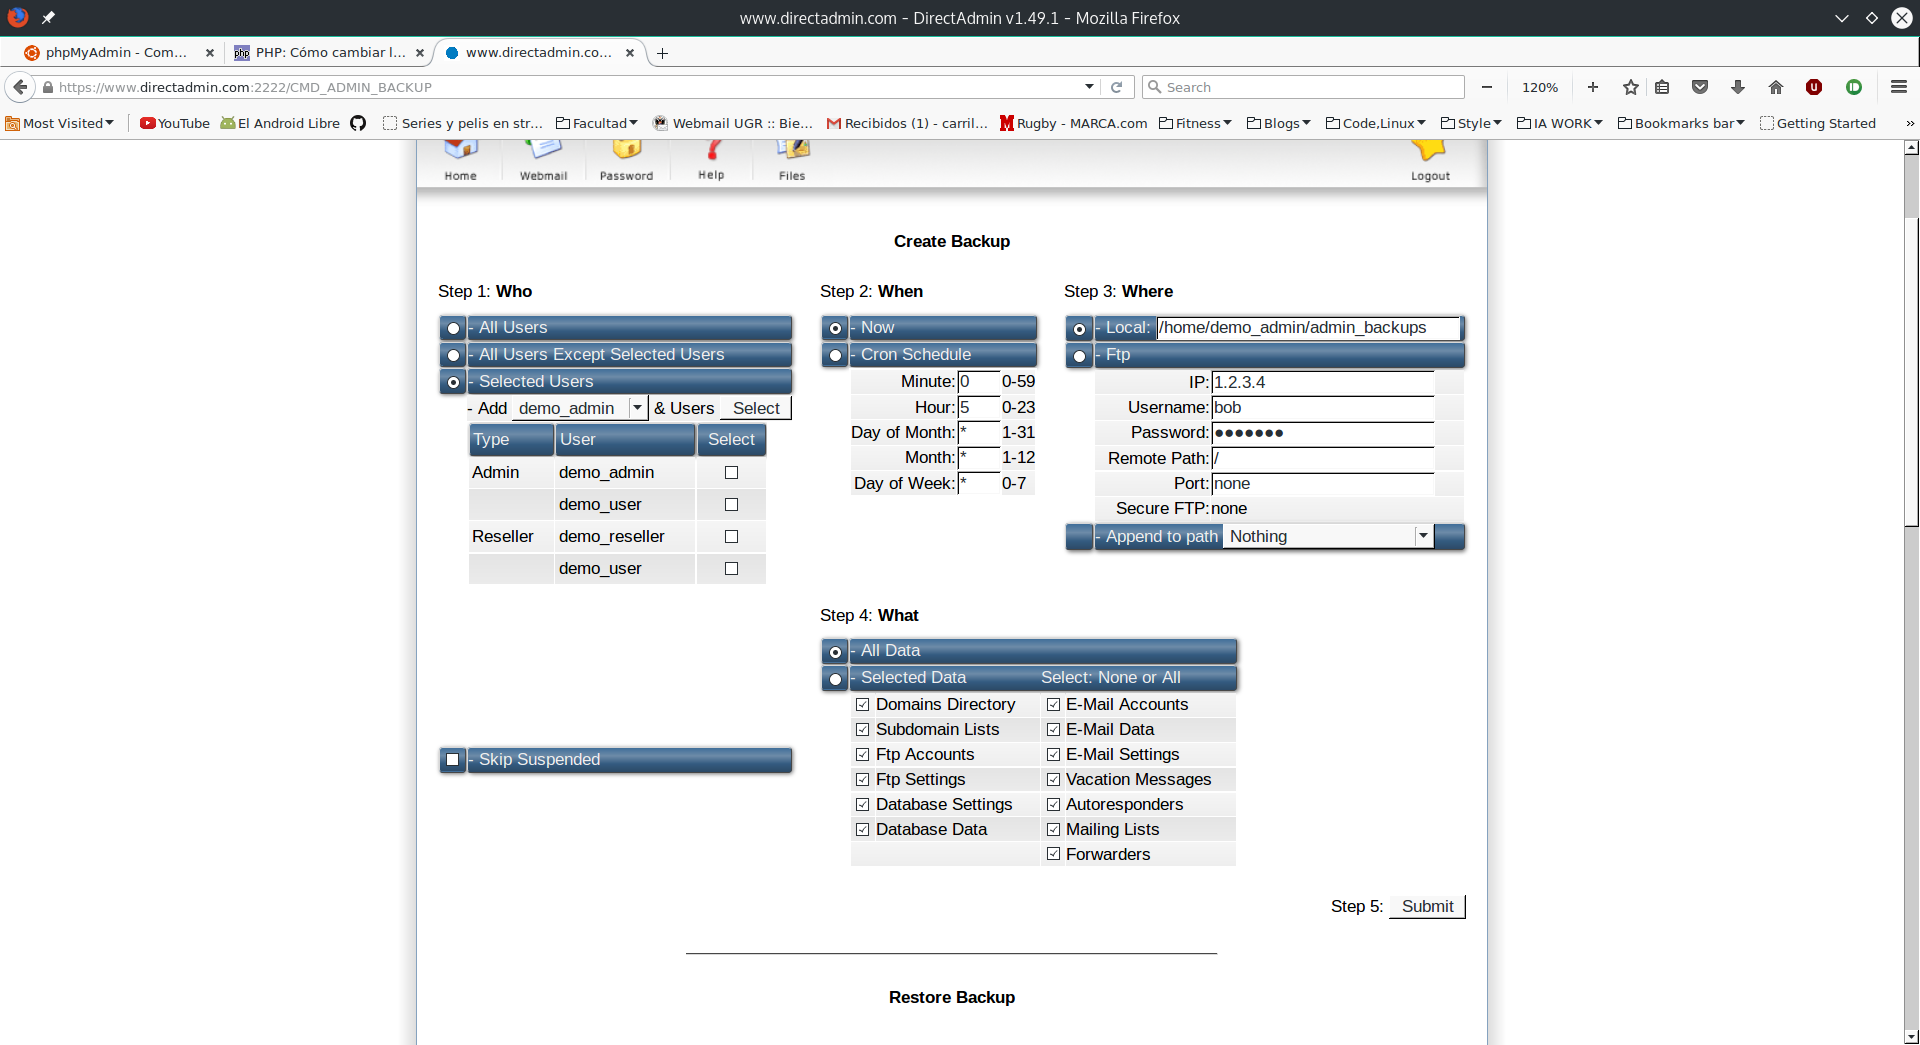
\includegraphics[scale=0.3]{figuras/figura19.png}  %el parámetro scale permite agrandar o achicar la imagen. En el nombre de archivo puede especificar directorios
	\label{figura19}
	
	\caption{Realizar backups pudiendo elegir los usuarios, crear un cron para que se ejecute cada x tiempo que le indiquemos, donde guardarlo y que guardar} 
\end{figure}

%%%%%%%%%%%%%%%%%%%%%%%%%%%%%%%%%%%%%%%%%%%%%%%%%%%%
% CUESTIÓN 17
%%%%%%%%%%%%%%%%%%%%%%%%%%%%%%%%%%%%%%%%%%%%%%%%%%%%

\section{Cuestión 17: Ejecute los ejemplos de find, grep y escriba el script que haga uso de sed para cambiar la configuración de ssh y reiniciar el servicio.}
Ejecutando el ejemplo del comando grep obtenemos el siguente resultado: 
\begin{figure}[H] %con el [H] le obligamos a situar aquí la figura
	\centering
	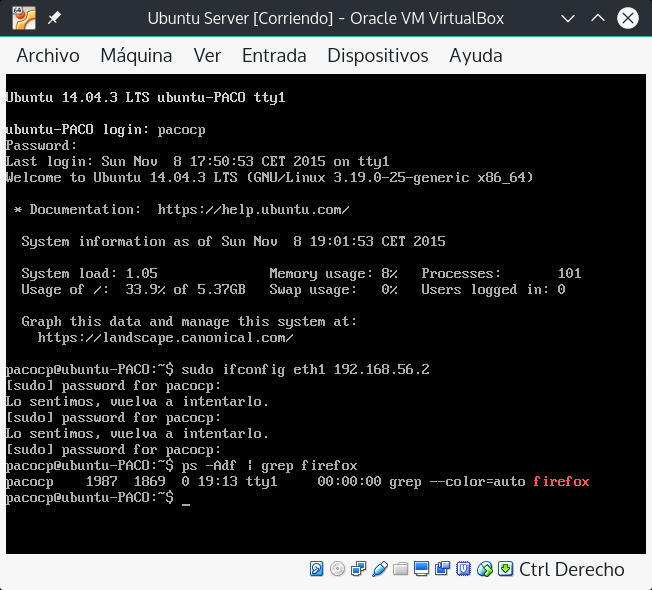
\includegraphics[scale=0.5]{figuras/figura20.png}  %el parámetro scale permite agrandar o achicar la imagen. En el nombre de archivo puede especificar directorios
	\label{figura20}
	
	\caption{Lo que obtenemos ejecutando el comando grep } 
\end{figure}
Ejecutando el ejemplo del comando find obtenemos el siguiente resultado:
\begin{figure}[H] %con el [H] le obligamos a situar aquí la figura
	\centering
	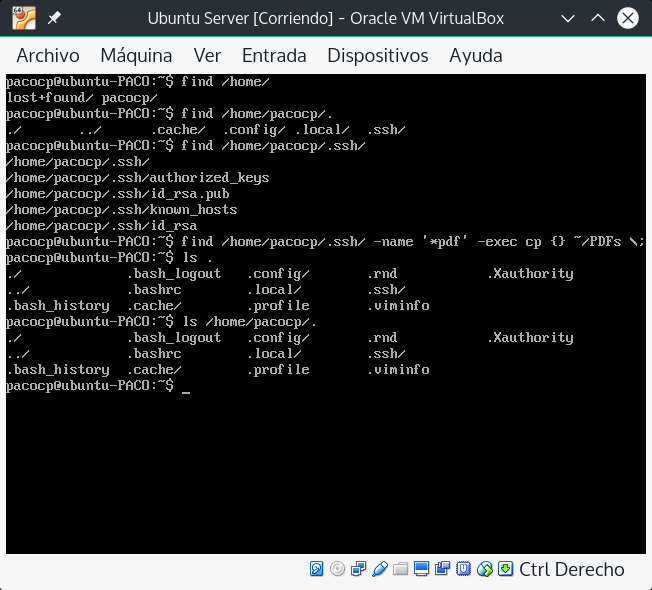
\includegraphics[scale=0.5]{figuras/figura21.png}  %el parámetro scale permite agrandar o achicar la imagen. En el nombre de archivo puede especificar directorios
	\label{figura21}
	
	\caption{Claramente no funciona ya que en la carpeta .ssh no se encuentra ningún archivo PDF por lo que no se copia nada } 
\end{figure}

El script sería:\\
\begin{lstlisting}
#!/bin/bash/

echo "CHANGING THE FILE..." 

sudo sed -i "PasswordAuthentication yes\c/PasswordAuthentication no"  /etc/ssh/sshd_config

echo "RESTARTING THE SERVICE..."

service ssh restart 

echo "WAITING FOR YOU..."

sleep 300

echo "CHANGING THE FILE AGAIN..."

sudo sed -i "PasswordAuthentication no\c/PasswordAuthentication yes"  /etc/ssh/sshd_config

echo "RESTARTING THE SERVICE..."

service ssh restart 

echo "GOODBYE!"

\end{lstlisting}

%%%%%%%%%%%%%%%%%%%%%%%%%%%%%%%%%%%%%%%%%%%%%%%%%%%%
% CUESTIÓN 18
%%%%%%%%%%%%%%%%%%%%%%%%%%%%%%%%%%%%%%%%%%%%%%%%%%%%
\section{Cuestión 18: Escriba el script para cambiar el acceso a ssh usando PHP o Python.}

\begin{lstlisting}[language=python]
#!/usr/bin/env python
# -*- coding:utf-8 -*-
from sys import argv
import subprocess

print("CHANGING THE FILE...\n")

subprocess.call(['sudo','sed', '-i', "PasswordAuthentication yes\c/PasswordAuthentication no", '/etc/ssh/sshd_config'])

print("RESTARTING THE SERVICE...\n")


subprocess.call(['servive','ssh','restart'])

print("WAITING FOR YOU...\n")

subprocess.call(['sleep','300'])

print("CHANGING THE FILE AGAIN...\n")

subprocess.call(['sudo','sed', '-i', "PasswordAuthentication no\c/PasswordAuthentication yes", '/etc/ssh/sshd_config'])

print("RESTARTING THE SERVICE...\n")


subprocess.call(['servive','ssh','restart'])

print("GOODBYE!\n")

\end{lstlisting}

\section{Cuestión 19: Abra una consola de Powershell y pruebe a parar un programa en ejecución (p.ej), realice capturas de pantalla y comente lo que muestra.}
Siguiendo los comandos que he consultado en la página \cite{powershell} voy a ilustrar con las siguientes imágenes como se para un proceso:
\begin{figure}[H] %con el [H] le obligamos a situar aquí la figura
	\centering
	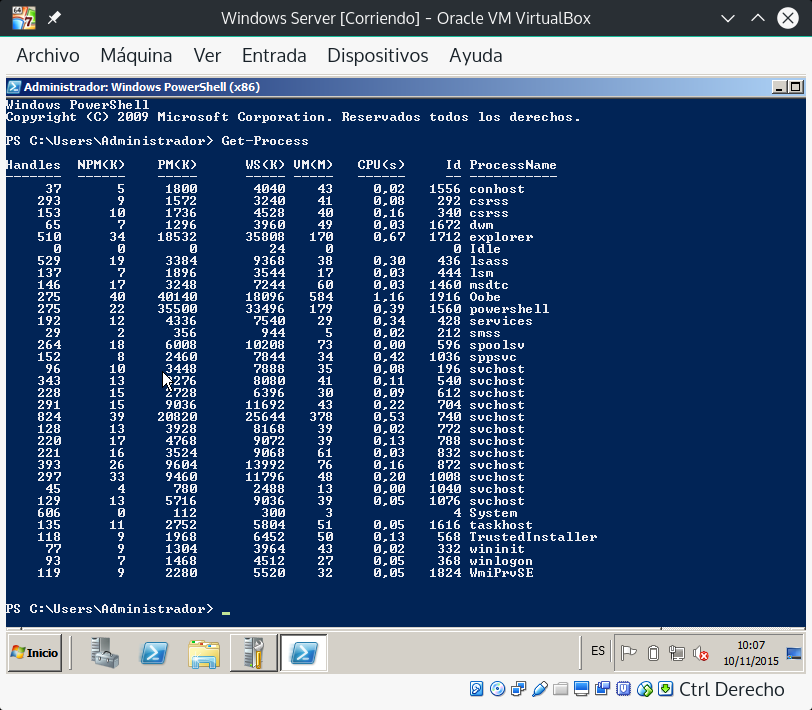
\includegraphics[scale=0.5]{figuras/figura22.png}  %el parámetro scale permite agrandar o achicar la imagen. En el nombre de archivo puede especificar directorios
	\label{figura22}
	
	\caption{Con el comando \textbf{Get-Process} obtenemos todos los procesos que se encuentran en ejecución en ese instante } 
\end{figure}
\begin{figure}[H] %con el [H] le obligamos a situar aquí la figura
	\centering
	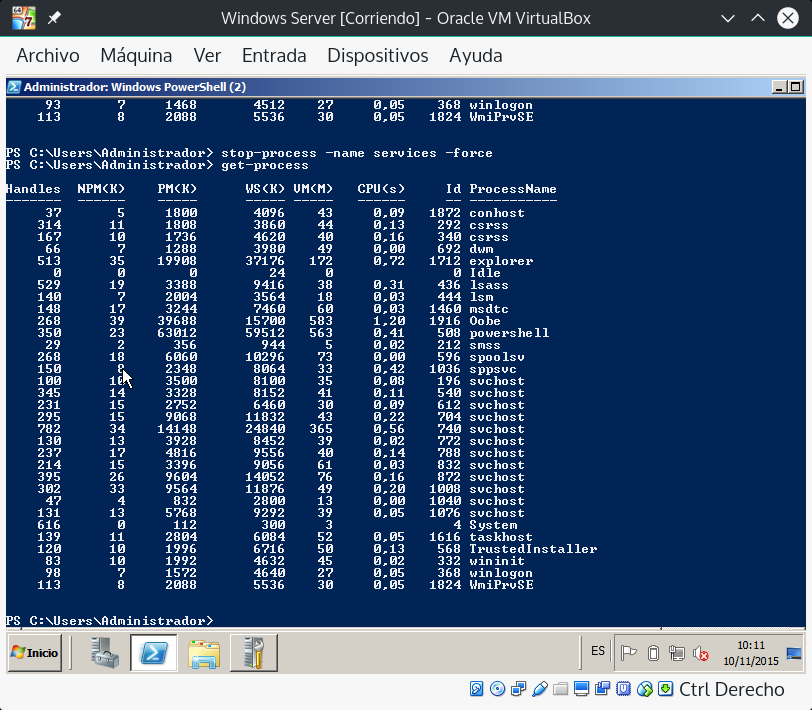
\includegraphics[scale=0.5]{figuras/figura23.png}  %el parámetro scale permite agrandar o achicar la imagen. En el nombre de archivo puede especificar directorios
	\label{figura23}
	
	\caption{Con el comando \textbf{stop-process -name services -force} paramos el proceso services forzándolo, ya que si no no se cierra. Podemos comprobar como se ha cerrado volviendo a ejecutar el comando \textbf{Get-Process} y comprobando que no se encuentra dentro de la lista.  } 
\end{figure}
\newpage
\bibliography{citas} %archivo citas.bib que contiene las entradas 
\bibliographystyle{ieeetr} % hay varias formas de citar
\end{document}